\documentclass[12pt,a4paper]{article} % Maybe use 'report' ???
% REMEMBER TO REMOVE THE 'draft' TAG!
\usepackage{polyglossia}	% XeTeX multi-lingual support
\usepackage{fontspec}		% The XeTeX font spec package
\usepackage{xunicode}		% XeTeX Unicode character support
\usepackage{xltxtra}		% Umm something else XeTeX

\usepackage[intlimits]{amsmath}	% Math stuff
%\usepackage{pdftexcmds} % pdf macros: needed for listingsutf8
\usepackage{listings}	% Package for code formatting
\usepackage[dvipsnames]{xcolor}
%\include{/home/johnlm/code/avr_assembler_listing_def.tex}
%\input{avr_assembler_listing_def.tex}
%\renewcommand{\lstlistingname}{Koda bloks}
\usepackage{longtable}	% Package for tables split accross pages
\usepackage{booktabs}	% Package for nicer tables
\usepackage{enumerate}
\usepackage[toc,title,titletoc]{appendix}
%\usepackage{wrapfig}
\usepackage{cite}	% Superscript cites
\usepackage{rotating}	% Package for landscape figures
\usepackage{indentfirst}	%Indent first paragraph too
\usepackage{setspace}	% Line spacing package
\usepackage[perpage,symbol*,bottom]{footmisc}	% Resets footnote marks per page
%NOTE: footmisc must load AFTER setspace
\usepackage{fancyhdr}	% Fancy header/footer package
\usepackage{placeins}
\usepackage[figurewithin=section,tablewithin=section]%
	{caption}	% Package for configuring captions format
\usepackage[a4paper,xetex,top=20mm, bottom=22mm, left=35mm, right=20mm]%
%\usepackage[a4paper,top=22mm, bottom=25mm, left=35mm, right=20mm]% DEBUG
	{geometry}

% Preamble formatting settings defined included from external file
% Polyglossia settings
\setmainlanguage{latvian}
\setotherlanguages{english,russian}

% FONTS (Empty \setmainfont gives you new Computer Modern)
% Deja Vu Family (rather good but wide chars)
%\setmainfont{DejaVu Serif}
%\setsansfont{DejaVu Sans}

% Liberation Family (my current favourite)
%\setmainfont{Liberation Serif}
%\setsansfont{Liberation Sans}

% Monos
%\setmonofont{DejaVu Sans Mono}

% Russian Font
%\newfontfamily\cyrillicfont{Liberation Serif}
\newfontfamily\cyrillicfont{CMU Serif}	% Unicode Computer modern font
%Other fonts are too "fat"/wide

%% Liberation Serif for VeA title font
\definecolor{SeaBlue}{cmyk}{1,0,0.37,0.52}
%% Use proper Aurora Bold Condensed BT
\newfontfamily\TitleFont[%
	Path = /home/johnlm/Development/resources/tex_graphics_lib/fonts/ ,%
	FakeStretch = 1.5 ,
	Color = SeaBlue
	]{aurora-BT-condensed-bold}

% External common image library
\graphicspath{{/home/johnlm/Development/resources/tex_graphics_lib/}{img/}}

\hyphenpenalty=7500
\clubpenalty=9000
\widowpenalty=9000

% Set rubberband values
\setlength{\parskip}{1ex plus 3ex minus 1ex}	% Space between paragraphs


%\renewcommand{\thefootnote}{\alph{footnote}} % Piezīmes ar burtiem
\newcommand{\citeet}[1]{\textsuperscript{\cite{#1}}}

%% Numbering format fix for sections and subsections (trailing full-stop)
%\def\thesection{\arabic{section}.}
%\def\thesubsection{\thesection\arabic{subsection}.}
% Add deeper levels if required
%% FIXED: fixlatvian.sty provides these (REMOVE THIS)

% Reformatting captions
\captionsetup{format=hang,font={small}}	% GLOBAL
%\captionsetup[table]{position=top,

% Footer adjustements (by redefining plain pagestyle)
\setlength{\headheight}{15.2pt}
\fancypagestyle{plain}{%
	\fancyhf{}	% Clear current (default) header/footer
	\rfoot{\thepage}	% Page number on outside
	\renewcommand{\headrulewidth}{0pt}
	\renewcommand{\headrulewidth}{0pt}}


% Other stuff
\newcommand{\todo}{\textcolor{red}{TODO}}

%% Inline Word inclusion formatting
\newcommand{\termEn}[1]{\textenglish{\itshape {#1}}} % inline English

% Superscript cite
\makeatletter
	\renewcommand\@citess[1]{\textsuperscript{[#1]}}
\makeatother




%% This file contains special, document-specific preamble settings
% Binary code formatting for instruction table
\newcommand{\instr}[7]{\texttt{%
	\textcolor{purple}{#1}%		Group OPCODE
	\textcolor{blue}{#2}%		Vector OPCODE (part 1)
	\textcolor{cyan}{#3}%		Vector OPCODE (part 2)
	\textcolor{lightgray}{#4}%		Middle Slack bits
	\textcolor{OliveGreen}{#5}%		Argument 1
	\textcolor{Green}{#6}%	Argument 2
	\textcolor{lightgray}{#7}}}%		Trailing Slack bits
\newcommand{\mnem}[1]{\texttt{\bfseries #1}}

%% listings definiicijas
\lstdefinelanguage[qucs]{VHDL}[]{VHDL}%
{%morekeywords=[1]{},% MOAR core keywords
morekeywords=[3]{ieee,std_logic_1164,std_logic_arith,std_logic_unsigned,%
	work,std,textio,numeric_std,% usual libraries
	std_logic,std_logic_vector,unsigned,signed,%logic data types
	time,integer,real,line,string,positive,natural,% data types
	ns},%real type units
morekeywords=[4]{reverse_range,length,event,last_value,high,low},% attributes
morekeywords=[5]{write,writeline,conv_integer,to_unsigned,rising_edge,falling_edge}%,%funkcijas
%morestring=[b]',
}

\lstdefinelanguage{JSI}%
 {morekeywords={LD,LDI,MOV,ST,AR,ADD,SUB,INC,DEC,AND,OR,XOR,NOT,CLR,%
	MOV,LSL,LSR,ROR,ROL,BREQ,BRNQ,BRGT,BRGE,BRLE,BRLT,HLT,JMP},%
morekeywords=[2]{DEVCTRL_REG_ADDR,SPI_RING_REG_ADDR,%
	BOOT_ROM_START,BOOT_ROM_END,%
	CONF_REG_START,CONF_REG_END,IO_MAP_START,IO_MAP_END,%
	SRAM_START,SRAM_END,SRAM_A_START,SRAM_A_END,SRAM_B_START,SRAM_B_END},% Ports and internal registers
morekeywords=[3]{def,include,equ,dw,org},% directives
morekeywords=[4]{DCR_SPI_WIDTH,SPI_16_MODE,SPI_8_MODE,%
	DCR_SPI_FLASH_EN},% header constants
   sensitive=true,%
   %morecomment=[l]*,%
   morestring=[b]",
   morecomment=[l];%
   }[keywords,comments,strings]



%% English determined number suffixes
%\renewcommand{\th}{\textsuperscript{th} }
\newcommand{\st}{\textsuperscript{st} }
\newcommand{\rd}{\textsuperscript{rd} }
\newcommand{\nth}{\textsuperscript{th} }


% Hyperref package for links in PDF (should be last package)
\usepackage[hyperfootnotes=false,linkbordercolor={blue},hyperindex]{hyperref}
\hypersetup{pdftitle={Iekļautās sistēmas mikrokontroliera kodola izstrāde}}
\hypersetup{pdfauthor={Jānis Šmēdiņš}}

\usepackage{fixlatvian}	% Fixes for Latvian typography rules


% \onehalfspacing

% Chardump: „” em— en– fig‒ “”
\begin{document}
	% Titullapa
	\pagestyle{empty}
	% LM izcilā VeA titullapa bakalauram!
\begin{titlepage}
	% VeA Logo
	% "Ventspils Austskola" virsraksts (\TitleFont jābūt definētam!!!)
	\newsavebox{\veatext}
	\savebox{\veatext}{
		\TitleFont\Huge\MakeUppercase{Ventspils Augstskola}}
	% Teksta platuma noteikšana (lai pielīdzinātu bildi tā platumam}
	\newlength{\veatextwidth}
	\settowidth{\veatextwidth}{\usebox{\veatext}}
	% Šeit drukāts pats logo un nosaukums
	\centering\includegraphics[width=0.98\veatextwidth]{VeA_logo.pdf}\\[4pt]
	\usebox{\veatext}\\[6pt]
	\large Informācijas tehnoloģiju fakultāte\\[2cm]
	
	\textbf{Bakalaura darbs}\\[1.5cm]
	%\textbf{Bakalaura darba 1.~atskaite}\\[1.5cm]
	
	\textsc{\LARGE Iekļautās sistēmas mikrokontroliera kodola izstrāde}
	\vfill % LIELĀ atstarpe
	
	%\raggedleft
	\normalsize
	\begin{minipage}[t]{0.4\textwidth}
		\begin{flushleft}
			Autors
		\end{flushleft}
	\end{minipage}
	\begin{minipage}[t]{0.55\textwidth}
		\begin{flushleft}
			Ventspils Augstskolas \\
			Informācijas tehnoloģiju fakultātes \\
			bakalaura studiju programmas „Elektronika”\\
			3. kursa students \\
			\textbf{Jānis Šmēdiņš}\\
			Matr.~nr.~\texttt{2009120280}\\
			\rule[-1em]{10em}{1pt}\\
			\makebox[10em][c]{\tiny (paraksts)}\\[1cm]
		\end{flushleft}
	\end{minipage}\\[2em]
	\begin{minipage}[t]{0.4\textwidth}
		\begin{flushleft}
			Fakultātes dekāns
		\end{flushleft}
	\end{minipage}
	\begin{minipage}[t]{0.55\textwidth}
		\begin{flushleft}
			asoc.prof.,~Dr.~math.~Gaļina Hiļķeviča\\[1ex]
			\rule[-1em]{10em}{1pt}\\
			\makebox[10em][c]{\tiny (paraksts)}\\[1cm]
		\end{flushleft}
	\end{minipage}\\[2em]
	\begin{minipage}[t]{0.4\textwidth}
		\begin{flushleft}
			Zinātniskais vadītājs
		\end{flushleft}
	\end{minipage}
	\begin{minipage}[t]{0.55\textwidth}
		\begin{flushleft}
			%asoc.prof.,~Dr.~math.~Gaļina Hiļķeviča\\
			\rule[-1em]{20em}{1pt}\\
			\makebox[20em][c]{\tiny
				(ieņemamais amats,
				zinātniskais nosaukums,
				vārds, uzvārds)}\\[1ex]
			\rule[-1em]{10em}{1pt}\\
			\makebox[10em][c]{\tiny (paraksts)}\\[1cm]
		\end{flushleft}
	\end{minipage}\\[2em]
	\begin{minipage}[t]{0.4\textwidth}
		\begin{flushleft}
			Recenzents
		\end{flushleft}
	\end{minipage}
	\begin{minipage}[t]{0.55\textwidth}
		\begin{flushleft}
			\rule[-1em]{20em}{1pt}\\
			\makebox[20em][c]{\tiny
				(ieņemamais amats,
				zinātniskais nosaukums,
				vārds, uzvārds)}\\[1ex]
			\rule[-1em]{10em}{1pt}\\
			\makebox[10em][c]{\tiny (paraksts)}\\[1cm]
		\end{flushleft}
	\end{minipage}\\[1cm]
	
	\centering
	Ventspils\\
	\the\year
\end{titlepage}
 % Ielikt titullapu
	\stepcounter{page} %Palielināt lapu skaitītāju (jeb ieskaitīt titullapu)
	
	%% Number listings within section
	% Add section number to caption
	\renewcommand{\thelstlisting}{\thesection.\arabic{lstlisting}}
	% Redefine \section to reset the lstlisting counter
	\let\oldSection\section
	\renewcommand\section{\setcounter{lstlisting}{0}\oldSection}
	
	%\renewcommand{\contentsname}%
	%	{\vspace*{-12mm}\section*{Saturs}\vspace*{-6mm}}
	\tableofcontents
	%\addcontentsline{toc}{section}{Saturs}	% Saturs ir saturaa?
	
	\clearpage
	\sloppy %Don't care too much about rigid formatting
	\onehalfspacing % 1.5 spacing
	
	% Termini
		% Seriālā, paralēlā datu pāraide
		% Mikrokontrolieris, uC
		% FPGA
		% SPI
		% ALU
		% boot
	
	%% Abstracts
% The 'abstract' enviroment makes more problems than it is useful

\phantomsection\addcontentsline{toc}{section}{\abstractname}
\abstitlestyle{\abstractname} % The abstract title (centered)
% Abstract text goes here
\noindent%
\begin{tabularx}{\textwidth}{lX}
	\textbf{Darba nosaukums:} & 
		\textit{Iekļautās sistēmas mikrokontroliera kodola izstrāde}\\[1ex]
	\textbf{Darba autors:} & Jānis Šmēdiņš\\[1ex]
	\textbf{Darba vadītājs:} & Mg.~sc.~comp.~Gatis Gaigals\\[1ex]
	\textbf{Darba apjoms:} & 68~lpp., 3~tabulas, 26~attēli,
		12~pirmkoda izdrukas, 19~bibliogrāfiskie avoti, 5~pielikumi\\[1ex]
	\textbf{Atslēgas vārdi:} & Mikrokontroliera kodols, aparatūras apraksta valodas,
		sintezējams mikrokontrolieris
\end{tabularx}

\vspace{1em}
Šī bakalaura darba mērķis ir izstrādāt modulāru mikrokontroliera kodolu,
kurš izmantojams dažādu, specializētu mikrokontrolieru implementācijās,
kuras bieži nepieciešamas specifiskos elektroniskajos risinājumos,
galvenokārt, zinātniskajos projektos. Mikrokontroliera un
izstrādātā kodola mērķa platforma ir FPGA.
%FIXME: Saīsinājuma atšifrējumu vajag uzrādīt?

Izstrāde veikta izmantojot aparatūras apraksta valodas, kas ir galvenais
FPGA projekta izstrādes instruments. Ir veikts divu galveno aparatūras
apraksta valodu (VHDL un Verilog) salīdzinājums, lai pamatotu izstrādes valodas izvēli.
Darbā analizēta eksistējoša procesora
arhitektūra, identificēti tās
trūkumi un izstrādāti uzlabošanas risinājumi, kā rezultātā izveidota 
bāzes arhitektūra, pēc kuras
realizēts izstrādājamais mikrokontroliera kodols.

Šī darba laikā kodols tika veiksmīgi izstrādāts, tā pārbaudei un 
demonstrācijai izstrādāts arī parauga mikrokontrolieris, kurā šis kodols
izmantots. Papildus izstrādāts asemblerkoda translators.
Izvirzīti vairāki priekšlikumi, kā uzlabot izstrādāto
mikrokontroliera kodolu.

\clearpage
\begin{english} % The English abstract
	\phantomsection\addcontentsline{toc}{section}{\abstractname}
	\abstitlestyle{\abstractname} % The abstract title (centered)
	% Abstract text goes here
	\noindent%
	\begin{tabularx}{\textwidth}{lX}
		\textbf{Title:} & 
			\textit{Development of embedded system microcontroller core}\\[1ex]
		\textbf{Author:} & Jānis Šmēdiņš\\[1ex]
		\textbf{Supervisor:} & Mg.~sc.~comp.~Gatis Gaigals\\[1ex]
		\textbf{Scope:} & ??~pages, ??~tables, ??~figures, ??~listings,
			??~bibliographical references, ?~appendices\\[1ex]
		\textbf{Keywords:} & Microcontroller core, hardware description languages,
				synthesisable microcontroller
	\end{tabularx}
	
	\vspace{1em}
	This bachelors thesis purpose is to develop a microcontroller core for
	synthesis on FPGA, as part of microcontroller, whether stand-alone or
	control device within special purpose integrated circuit.
	The thesis also focuses on hardware description languages
	(HDL) as a main tool of attaining this goal.
	
	The author takes a more practical approach by developing first and
	addressing problems as they arise. The work used an existing
	architecture of central processing unit as base which was then improved
	and modified in successive, iterative development cycles
	(dubbed revisions), where each such cycle is to result in a working
	prototype.
	
	During the development the instruction set of core was completely
	revised and several notable architectural changes done, most evidently
	the internal data bus was reimplemented as one-way, branched, circular
	pipeline. The author successfully developed a synthesisable
	microcontroller core which is the result of third development cycle (rev.~03).
	For testing	and demonstration purposes a complete microcontroller prototype
	incorporating the core was developed as well.
	
	The author proposes several possible improvements for a
	potential next development cycle, but also acknowledging that there
	could be indefinite number of such cycles, and that one fulfilling
	requirements will suffice.
	
	%%%%%%%%%%%%
	%This bachelors thesis focuses on an existing architecture of 
	%central processing unit	prototype. The author analyses the architecture,
	%identifying design flaws and suggesting solutions to these flaws.
	%These solutions are put to practical use by developing a
	%synthesisable microcontroller core (essentialy a CPU),
	%improving upon the existing	architecture.
	
	%To demonstrate use of the developed microcontroller core, a prototype
	%microcontroller is developed as well, which incorporates the core.
	
	%Hardware description languages are analysed as well, of which the VHDL
	%is used as a main tool of development. A short introduction and
	%analysis is done on FPGAs, which is the target platform for design
	%synthesis.
\end{english}

\clearpage
\begin{russian} % The Russian abstract
	\phantomsection\addcontentsline{toc}{section}{\abstractname}
	\abstitlestyle{\abstractname} % The abstract title (centered)
	% Abstract text goes here
	\noindent%
	\begin{tabularx}{\textwidth}{lX}
		\textbf{Название работы:} & 
			\textit{Разработка ядра микроконтроллера во встроенной системы}\\[1ex]
		\textbf{Автор работы:} & Jānis Šmēdiņš (транслит.~Янис Шмэдиньш)\\[1ex]
		%\textbf{Руководитель работы:}
		\textbf{Руководитель:} & Mg.~sc.~comp.~Gatis Gaigals 
			(транслит.~Гатис Гайгалс)\\[1ex]
		\textbf{Размер:} & 68 стр., 3 таблицы, 26 изображений,
			12 листингов (печатей исходного кода), 19 библиографических источников, 5 приложений\\[1ex]
		\textbf{Ключевые слова:} & ядро микроконтроллера,
			языки описания аппаратуры, синтезируемый микроконтроллер
	\end{tabularx}
	
	
	Цель работы бакалавра разработать модулярное ядро микроконтроллера
	которого можно использовать в разных специализированных имплементациях
	микроконтроллеров которые часто нужны в специфичных электронных решениях,
	восновном, в научных проектах. Целевой платформой микрокотроллера и
	разработанного ядра является FPGA.

	Разработка сделана, используя языки описания аппаратуры, которые
	являются главным инструментом проекта FPGA. Сделано сравнение двух
	главных языков описания аппаратуры (VHDL и Verilog), что-бы основать
	выбор языка разработки. В работе анализируется архитектура существующего
	процесора, идентифицированы недостатки и разработаны способы улучшения,
	в результате сделана базовая архитектура, по которой реализовано
	ядро разрабатываемого микроконтроллера.

	Во время этой работы ядро было успешно разработано, для его
	проверки и демонстрации  тоже разработан образцовый микроконтроллер,
	в котором это ядро будет использоватся. Дополнительно разработан
	транслятор кода ассемблера. Выдвинуто несколько предложений,
	как улучшить разрабатываемое ядро микроконтроллера.
	
\end{russian}

	
	% Ievads
	\clearpage
	\pagestyle{plain} % Start the proper page numbering
	\section*{Ievads} \addcontentsline{toc}{section}{Ievads}
Šis darbs apraksta mikrokontroliera kodola un tā perifērijas izveidi
funkcionālai parauga mikrokontroliera realizācijai. \todo

% TODO: Potenciālais pielietojums
	
	VHDL apraksta valodā. Izklāstītā informācija balstīta vairāk uz
	praktiskā darba rezultātiem un tādējādi arī darba gaitā pieņemtajiem
	lēmumiem sastapto problēmu risinājumam.
	
	Apskatīta procesora uzbūve bez kopējās datu šinas un reducētu instruk\-ciju
	kopu, realizācijai uz FPGA čipa platformas — konkrēti,
	\termEn{Actel Fusion Embedded Development Kit} ar \texttt{M1AFS1500}
	FPGA čipu. Darba mērķi tātad ir:
	\begin{itemize}
		%\item Funkcionāla procesora izstrāde VHDL;
		%\item Perifērijas izstrāde sintezējamai sistēmai;
		%\item Sistēmas sintēze un pārbaude.
		\item \todo
	\end{itemize}
	
	Darba gaitā pieņemtie lēmumiem, kas ievērojami izmaina sistēmas
	imple\-men\-tā\-ciju un ir izstrādes pagrieziena punkts, nosauktas par
	„Revīzijām”.
	Lai gan pamatā darbs atspoguļo galējo rezultātu, nodaļu
	beigās pievienots pārskats par Revīziju vēsturi — to iespaids uz
	izstrādi, kā arī šo izmaiņu pieņemšanas iemesli.
 % TODO: Rewrite this bugger
	
	% Teorija
	\clearpage
	%\section{Mikrokontrolieri} %TODO: Normālu nosaukumu?
%\todo

%Dzirdot vārdu ,,mikroprocesors'' un ,,datorsistēma'' vairums cilvēku 
%iztēlojas personālos datorus un klēpjdatorus, kas arī pēdējos gados ir teju
%vai katram. Tā gan ir tikai --- tēlaini izsakoties --- aisberga redzamā
%daļa. Mūsdienās mikroprocesori atrodami ļoti plaša klāsta dažādās sadzīves
%un industriālās ierīcēs, piem.~automašīnu elektronikā, ražošanas iekārtās,
%datortīklu maršutētājos, elektromēriekārtās, mobilajos telefonos,
%veļas mašīnu kontroles blokos un pat rotaļlietās.\cite[1.~lpp.]{Heath}

%% TODO: Šito mošk vajag pārfrāzēt
%Iekļautā sistēma arī ir datorsistēma, kuras primārā atšķirība no 
%vispārēja pielietojuma datorsistēmas ir darba specializācija,
%no kā seko praktiski visas realizācijas atšķirības. \todo

%TODO?: Procesors

\section{Aparatūras apraksta valodas}
Šajā darbā mikrokontroliera kodols un paraugimplementācija izstrādāta
galvenokārt izmantojot aparatūras apraksta valodu, un tādēļ lai radītu
priekšstatu par darba metodiku, šī nodaļa apskata 
aparatūras apraksta valodas, to īpašības un pielietojumu.

Elektronikai attīstoties un paaugstinoties tirgus prasībām produkta funkcionalitātei,
izstrādājamās sistēmas kļūst aizvien sarežģītākas. Jo sevišķi komplicētu ciparu shēmu, 
kā piemēram mikroprocesoru, iekšējo uzbūvi izstrādāt tradicionālā ceļā,
shematiski attēlojot komponentes un to savstarpējos savienojumus, kļūst
nepraktiski. Aparatūras apraksta valodas, savukārt, piedāvā augstākas
abstrakcijas izstrādes modeli, kas saīsina izstrādes laiku.
% [\todo{}?]. % Citation needed

Aparatūras apraksta valoda jeb HDL
(no angļu \termEn{Hardware description language})
ir valoda, ar kuras izteiksmēm, sekojot konkrētās 
valodas sintaktiskajiem nosa\-cī\-jumiem, ir iespējams aprakstīt
izstrādājamās shēmas uzbūvi un darbību \cite{HDL}. %Šo aprakstu dēvē par ,,kodu''.
HDL gandrīz vienmēr (bet ne obligāti) apraksta ciparu shēmas.
Līdzīgi program\-mē\-šanas valodām, HDL piedāvā dažādas sintaktiskās 
konstrukcijas, kas ļauj strukturēt aprakstu un veikt abstrakcijas,
ar kurām iespējams kompakti aprakstīt sarežģītas shēmas
\cite[1.~lpp.]{Perry-VHDL}.
Savukārt, atšķirībā no vairuma programmēšanas valodu,
izpildāmās izteiksmes ir ,,konkurentas'', t.i.,~tās tiek izpildītas paralēli, 
tādējādi shēmas definējošā apgabala izteiksmju secība ir maznozīmīga%
\footnote{Izteiksmju secībai ir nozīme secīgajās konstrukcijās.
	(sk.~\ref{sec:hdl-styles}~nod.)}.

HDL apraksti ir mašīn\-apstrādājami, kas dod iespēju izmantot
HDL simulācijas rīku, lai varētu veikt HDL aprakstītās shēmas 
darbības simulāciju, t.i.,~programmatūras līmenī 
atveidota aprakstītās shēmas darbība, no kuras iegūstamas jebkuru
shēmas signālvadu laika oscilogrammas, atmiņas elementu saturs un to izmaiņas,
kā arī iespējams citi dati. Analizējot simulācijas rezultātus ir 
iespējams pārbaudīt aprakstītās shēmas darbības korektumu pirms
tās fiziskās realizācijas. Iespēja simulēt HDL aprakstu ir ievērojama
priekšrocība izstrādei ar HDL.

Tomēr galvenais iemesls HDL izmantošanai un popularitātei ir iespējai veikt 
shēmu sintēzi --- automatizētu fiziskās realizācijas ģenerēšanu pēc HDL apraksta
\cite{HDL}\cite{Perry-VHDL}\cite{Vahid-RTL}. Tieši HDL aprakstu sintezējamība ir
īpašība, kas padara izstrādi ar HDL rūpnieciski nozīmīgu.
HDL pieraksta nianses sintēzei tiks apskatītas sekojošā \ref{sec:hdl-styles}~%
nodaļā, bet konkrētās sintēzei izmantotās tehnoloģijas --- 
\ref{sec:synth}~nodaļā (\pageref{sec:synth}~lpp.).

Eksistē daudz aparatūras apraksta valodu, gan valodas, kas izveidotas
speciāli aparatūras aprakstam, gan speciālas pakotnes, kuras pielāgo
eksistējošas programmēšanas valodas aparatūras aprakstam.
Tomēr nozarē svarīgākās ir VHDL un ,,Verilog'', kas ir arī
vienas no vecākajām un visvairāk attīstītajām HDL.
Šīs valodas īsumā tiek apskatītas \ref{sec:vhdl}~un \ref{sec:verilog}~%
nodaļā, un to salīdzinājums --- \ref{sec:hdl-comparison} nodaļā.

\subsection{Aprakstu stili} \label{sec:hdl-styles}
Vienādas komponentes HDL parasti var aprakstīt vairākos veidos.
HDL aprakstus var sadalīt divos pieraksta stilos, pēc problēmas pieejas un
no valodas konstrukciju kopas kas šai pieejai raksturīga.
\begin{enumerate}
	\item \textbf{Strukturālais} pieraksta stils --- komponentes tiek
		izveidotas izmantojot vienkāršākas apakškomponentes un aprakstot 
		to savstarpējos
		savienojumus. Šis stils uzskatāms par tekstuālu analogu
		tradicionālajam, shematiskajam izstrādes veidam.
	\item \textbf{Funkcionālās} jeb izturēšanās modelēšanas pieraksta
		stils --- komponentes tiek izveidotas aprakstot shēmas funkcionalitāti
		abstrahējoties no tās iespējamās uzbūves.
	\begin{itemize}
		\item \textbf{Secīgās izturēšanās} pieraksta stils --- apakškopa
			no funkcionālā stila, kurā izmantotas konstrukcijas, kas ļauj
			komponentes darbību aprakstīt ar secīgām izpildāmām izteiksmēm,
			līdzīgi imperatīvām programmēšanas valodām (kā C, Python, u.c.),
			pretstatā paralēli izpildāmām datu plūsmas izteiksmēm.
	\end{itemize}
\end{enumerate}
\pagebreak[3]

Šie stili ne tikai ietekmē koda (konkrētā shēmas apraksta teksta) pierakstu,
bet arī simulācijas un sintēzes procesus, kuriem šis pieraksts ir jāinterpretē.
Strukturālā pieraksta un tādu funkcionālā pieraksta primitīvu konstrukciju,
kā loģisko elementu (\texttt{UN}, \texttt{VAI}, utt.)
sintēze ir tieši translējama uz aparatūras komponentēm un to savienojumiem.
Savukārt, sarežģītu funkcionālo konstrukciju (jo sevišķi secīgo
konstrukciju) sintēzei nepieciešams veikt speciālu funkcionalitātes apraksta
translāciju uz konkrētu aparatūras implementāciju, t.i.,~sintēzes rīkam nepieciešams
piemeklēt aparatūras komponentes, kas realizētu konkrēto funkcionalitāti.
Tā kā funkcionalitātes un implementācijas saistība bieži nav viennozīmīga,
dažādu sintēzes rīku interpretācija vienādam kodam var stipri atšķirties.

Praktiski visi sintēzes rīki funkcionālo pierakstu translē %uz aparatūras 
reģistru datu pārraides abstrakcijas līmenī jeb RTL
(no angļu \termEn{Register tranfer level}) \cite[2.~lpp.]{HDL}%
\cite[235.~lpp.]{Perry-VHDL}.
RTL abstrakcijas vienību (elementu) veido kombinacionālās datu transformācijas shēma un
datu uzglabāšanas reģistrs (sk.~\ref{fig:rtl}~att.).
\begin{figure}[thb]
	\centering
	%\def\svgwidth{7cm}
	\def\svgscale{1.25}
	\input{img/rtl-unit.pdf_tex}
	\caption[RTL abstrakcijas vienība.]{RTL abstrakcijas vienība \cite[233.~lpp.]{Perry-VHDL}.}
	\label{fig:rtl}
\end{figure}
Izstrādājot ierīci sintēzei ar HDL kodu, tiek bieži pieminēts
,,RTL apraksta stils''. Šis stils ir HDL konstrukciju kopa, kas
pakļaujas sintēzei un iekļauj visas strukturālā stila konstrukcijas, kā arī
lielu daļu funkcionālā stila konstrukcijas.

Jāuzsver gan, ka RTL pieraksta stils nepieprasa, lai katrai aprakstītai
komponentei būtu piekārtojams tieši viens RTL elements. Vienas komponentes
apraksts var saturēt vairākus RTL elementus, kā arī viens RTL elements var
pārklāt vairākas komponentes. Kā piemēru pēdējam variantam, var apskatīt
darba praktiskajā daļā izstrādāto mikrokontroliera datu kalkulācijas
signālceļu (sk.~\ref{fig:rtl-alu}~att.).
\begin{figure}[thb]
	\centering
	\def\svgwidth{0.9\textwidth}
	%\def\svgscale{1.25}
	{\ttfamily\scriptsize\input{img/rtl-alu.pdf_tex}}
	\caption{RTL sadalījuma piemērs ALU signālceļam.}
	\label{fig:rtl-alu}
\end{figure}
Šeit \texttt{alu} (Aritmētiski loģiskā ierīce) un \texttt{shift}
(Bitu bīdes loģiskā ierīce) ir kombinacionālās shēmas, bez iekšējiem atmiņas
elementiem, savukārt \texttt{reg} (Reģistrs), kura uzdevums ir saglabāt kalkulācijas
rezultātu, acīmredzami, ir reģistra jeb atmiņas daļa šajā RTL elementa piemērā.
Tādējādi šīs trīs komponentes veido vienu RTL elementu.

Konstrukcijas, kuras nav translējamas RTL, sauc --- visai aprakstoši --- par 
,,tikai simulējamām konstrukcijām''. Tās nav sintezējamas un tiek
izmantotas simulācijas ietvaros. Viena no vienkāršākajām un biežāk
izmantotajām ir novēlotā signāla piešķire, piem.,~VHDL izteiksme 
|q <= a after 10 ns;| piešķir |a| vērtību signālam |q| pēc 10 nanosekundēm.
Tas ir labs veids, kā simulēt komponenšu aiztures, bet tiks ignorēta
sintēzē, jo elementiem, ar kuriem tiks realizēta shēma, piemīt
konkrēta aizture, ko nosaka to fiziskā uzbūve.

Svarīgi piezīmēt, ka pretstatā sintēzes rīkam, simulatoram nav nepieciešama
pieraksta translācija RTL. Tā kā simulācija notiek
programmatūras līmenī, vairumā gadījumu secīgās izturēšanās modeli
simulatoram ir vienkāršāk (un tādējādi arī ātrāk) simulēt nekā paralēli
izpildāmās konkurentās konstrukcijas.
 \clearpage %\pagebreak[3]
\subsection{VHDL} \label{sec:vhdl}
	VHDL (no angļu \termEn{VHSIC hardware description language}) ir aparatūras apraksta
	valoda, kura ieviesta 1980-ajos gados Amerikas Savienoto Valstu
	Aizsardzības ministrijas
	VHSIC (\termEn{very-high-speed integrated circuits})
	projekta ietvaros \cite[141.~lpp.]{VHSIC}\cite[1.~lpp.]{Perry-VHDL}.

	VHDL sintakse ir modelēta pēc Ada programmēšanas valodas sintakses, kur
	valodas konstrukcijas un to semantiskā nozīme pielāgota aparatūras aprakstam.
	VHDL sintakse tiek uzskatīta par visai izsmeļošu, t.i.,~valodas 
	konstrukcijas un izteiksmes ir pierakstāmas visai gari, kas seko no
	Ada sintakses, kā arī fakta, ka VHDL sākotnēji bija paredzēta kā 
	formāla valoda komponenšu dokumentācijai, kas viennozīmīgi aprakstītu
	komponenšu darbību.
	VHDL apraksti papildināja komponenšu dokumentāciju,
	aizstājot komplicēto un, bieži vien,
	nekonkrēto vai neviennozīmīgo rakstveidā dokumentēto darbības modeli.
	
	Tā kā VHDL apraksti seko noteiktai striktai, viennozīmīgai sintaksei,
	tie ir mašīnlasāmi un tika izstrādāta programmatūra, kas deva
	iespēju veikt aprakstītās shēmas simulāciju un vēlāk arī sintēzi.

	\begin{lstlisting}[language={[qucs]VHDL},label=kb:vhdl-example,gobble=4,%
			caption={VHDL apraksts loģiskajam \texttt{UN} elementam.}]
		-- This adds IEEE library and nine-valued logic
		library ieee;
		use ieee.std_logic_1164.all;
		
		entity andgate is
			port ( A : in std_logic;
			       B : in std_logic;
			       Q : out std_logic );
		end entity andgate;
		
		architecture rtl of andgate is
		begin
			Q <= A and B; -- Simply 'AND' the inputs and output result
		end architecture rtl;
	\end{lstlisting}

	Vienkāršs loģiskā elementa \texttt{UN} VHDL apraksta paraugs redzams
	\ref{kb:vhdl-example}~pirmkoda izdrukā. Piemērā redzami pamata sintaktiskās
	konstrukcijas komponentes aprakstam.
	Pirmkārt, entītija definē aprakstāmās komponentes ,,no ārpuses''
	redzamās daļas, no kurām svarīgākā (un piemērā vienīgā) ir pieslēgvietu
	saraksts; otrkārt, arhitektūra ir komponentes implementācijas definīcija,
	kurā tiek aprakstīta entītijā definētās komponentes darbība.

	Tā kā izmantojot aprakstīto komponenti hierarhiālā shēmas projektēšanā, 
	galvenokārt ir svarīga komponentes darbība, nevis tās konkrētā implementācija,
	VHDL apraksta arhitektūru var uzskatīt par ,,slēpto'' vai ,,privāto''
	komponentes daļu.

	VHDL iebūvētais \texttt{bit} tips (kas pieņem tikai |0| vai |1| vērtības)
	nevar parādīt tādus aparatūras loģikas stāvokļus, kā augstas impedances
	(|Z|) stāvoklis, atsaites rezistoru ,,vājos'' loģikas līmeņus un nezināmu
	(|X|) loģisko stāvokli. Šo problēmu atrisina IEEE 1164 standarts, kurš definē
	\texttt{std\_logic} tipu ar deviņiem dažādiem stāvokļiem:
	\begin{itemize}
		\item \verb|'U'| --- neinicializēta (nezināma) loģiskā vērtība;
		\item \verb|'X'| --- nezināma loģiskā vērtība no spēcīga devēja;
		\item \verb|'0'| --- loģiskā 0 no spēcīga devēja;
		\item \verb|'1'| --- loģiskais 1 no spēcīga devēja;
		\item \verb|'Z'| --- augstas impedances stāvoklis (nav devēja);
		\item \verb|'W'| --- nezināma loģiskā vērtība no vāja devēja;
		\item \verb|'L'| --- loģiskā 0 no vāja devēja (piem.,~atsaites rezistors pret zemi);
		\item \verb|'H'| --- loģiskais 1 no vāja devēja (piem.,~atsaites rezistors pret barošanas spriegumu);
		\item \verb|'-'| --- ignorējama vērtība (\termEn{don't care})%
			\footnote{Vērtību \verb|'-'| var izmantot salīdzināšanā,
				lai ignorētu konkrētus bitus no bitu vektora.},
	\end{itemize}
	kā arī definē operācijas ar \texttt{std\_logic} tipa signāliem vai mainīgajiem. 
	Praktiski visi VHDL simulācijas rīki šo bibliotēku piedāvā.
	
	Sintēzes rīki arī atbalsta \texttt{std\_logic} tipu, bet ne visas
	\texttt{std\_logic} tipa pieņemamās vērtības ir sintēzei saistošas.
	Reālu ciparu shēmu ieejas signāls vienmēr tiks interpretēts kā |0| (zems līmenis) 
	vai |1| (augsts līmenis), un izejas var pieņemt |0|, |1| vai augstas
	impedances (|Z|) stāvokli. Izvadīt nezināmu (|X|) loģisko vērtību
	fiziskai komponentei nav iespējams.	%\todo{}?
	% TODO: Uztais normālu nobeigumu

\pagebreak[3]
\subsection{Verilog} \label{sec:verilog}
	Verilog ir aparatūras apraksta valoda, kuru 1980-ajos gados izstrādāja
	\termEn{P.~Moorby} un \termEn{P.~Goel}. Verilog sintakse ir daļēji modelēta
	pēc C programmēšanas valodas sintakses, kas papildus faktam, ka Verilog
	jau sākotnēji izstrādāta shēmu simulācijai, nevis
	kā formāla shēmu apraksta valoda, padara Verilog pierakstu visai kompaktu.

	\begin{lstlisting}[language={Verilog},label=kb:verilog-example,gobble=4,%
			caption={Verilog apraksts loģiskajam \texttt{UN} elementam.}]
		module andgate(A, B, Q);
			input A;
			input B;
			output Q;
			// inputs and outputs are of 'wire' type
			// unless redeclared otherwise
			
			assign Q = A & B; // Simply 'AND' the inputs and output result
		endmodule
	\end{lstlisting}

	Vienkāršs loģiskā elementa \texttt{UN} Verilog apraksta paraugs redzams
	\ref{kb:verilog-example}~pirmkoda izdrukā.
	Verilog modulis ir konstrukcija kas satur komponentes aprakstu
	--- gan ārējo saskarni, gan implementāciju.
	
	Verilog moduļus var izmantot citu moduļu definēšanā, tādējādi veicot
	hierarhiālu shēmas projektēšanu, bet Verilog neatbalsta pakotnes vai
	bibliotēkas konceptu, tādēļ moduļu otreizēja izmantošana citos projektos
	ir apgrūtināta.
	
	Verilog datu tipi, atšķirībā no VHDL, ne tikai izsaka
	to pieņemamās vērtības, bet arī to semantisko nozīmi shēmā
	\cite[21.~lpp.]{Vivek-Verilog}. Piemēram,
	gan \texttt{wire} (apakštips no \texttt{net}), gan \texttt{reg} tips
	satur četru stāvokļu loģikas datus, bet \texttt{wire} apzīmē
	apzīmē savienojumu mezglu (\termEn{net}), savukārt, \texttt{reg}
	vairumā gadījumu (bet ne obligāti) apzīmē atmiņas elementu (trigeri).
	Verilog četri loģiskie stāvokļi ir:
	\begin{itemize}
		\item |0| --- loģiskā 0, zems līmenis;
		\item |1| --- loģiskais 1, augsts līmenis;
		\item |z| --- augstas impedances stāvoklis;
		\item |x| --- nezināma loģiskā vērtība.
	\end{itemize}
	
	Verilog četru stāvokļu loģikas iespējamās vērtības neiekļauj
	,,vājos'' loģiskos stāvokļus, bet tos iespējams izteikt izmantojot
	\texttt{wire} tipa devēja stipruma uzstādījumu. \ref{kb:nand-oc}~kods
	parāda vienu no iespējamiem veidiem, kā aprakstīt \texttt{UN-NĒ}
	elementu ar atvērtā kolektora izeju, kuram pievienots atsaites rezistors
	pret barošanas avotu.
	\begin{lstlisting}[language={Verilog},label=kb:nand-oc,gobble=4,%
			caption={Verilog pieraksta paraugs devēja stipruma uzstādījumam.}]
		module nand_resistive_high(A, B, Q);
			input A;
			input B;
			output Q;
			// This emulates an open-collector output
			// with a pull-up resistor to Vcc
			wire (pull1, strong0) tmp;
			
			assign tmp = ~(A & B);
			assign Q = tmp;
		endmodule
	\end{lstlisting}
	
	Fakts, ka Verilog sākotnēji izstrādāts shēmu sintēzei, atstājis iespaidu
	uz valodas pieraksta sintezējamību. Verilog var aprakstīt sarežģītas
	sintezējamas shēmas ne sliktāk par citām HDL, bet eksistē virkne
	nosacījumu apraksta sintezējamības nodrošināšanai \cite{ieee-1364.1},
	kuri ir vairāk nekā citām HDL.
	

%\subsection[SystemC]{SystemC \textcolor{red}{???}}
	%\todo ?

\clearpage
\subsection{Valodu salīdzinājums} \label{sec:hdl-comparison}
	Ciparu elektronikas industrijā VHDL un Verilog ir visplašāk izmantotās
	HDL. Tā kā vairums FPGA un ASIC ražotāju (sk.~\ref{sec:synth}~nod.)
	piedāvātie izstrādes rīki atbalsta abas valodas, izvēles kritērijs
	valodas atbalstam ir kļuvis mazsvarīgs.
	
	Viena no būtiskākajām atšķirībām starp VHDL un Verilog ir datu tipu
	konversija. VHDL objektiem (pieslēgvietām, signāliem un mainīgajiem)
	piešķirama tikai vērtība, kas atbilst konkrētā objekta tipam
	(jāsakrīt gan tipam, gan vektoru garumiem)~\cite{vhdl-vs-verilog}.
	Ja nav tiešas atbilstības
	nepieciešams izmantot konversijas funkcijas vai citus pārvei\-do\-jumus,
	pat ja šo tipu sintēzes fiziskā realizācija ir identiska.
	Savukārt, Verilog
	dažāda garuma bitu vektori un \texttt{integer} tipa vērtības tiek
	savā starpā pārveidotas bez speciāla pieraksta pēc noklusējuma~\cite{vhdl-vs-verilog}.
	Abām pieejām ir 
	ieguvumu un trūkumi. ,,Nestingrajā'' tipu sistēmā iespējams īsāks un,
	iespējams, pārskatāmāks pieraksts, savukārt, ,,striktā'' tipu sistēma
	var novērst kļūdas, kas varētu rasties tipu pārveidošanas rezultātā,
	piem.,~bitu atmešana dažāda garuma bitu vektoru piešķirēs vai nekorekta
	zīmes bita interpretācija.
	
	\begin{figure}[thb]
		\centering
		\def\svgwidth{\textwidth}
		\input{img/hdl-abstractions.pdf_tex}
		\caption[VHDL un Verilog modelēšanas abstrakciju līmeņu salīdzinājums.]%
		        {VHDL un Verilog modelēšanas abstrakciju līmeņu salīdzinājums \cite{vhdl-vs-verilog}.}
		\label{fig:abstractions}
	\end{figure}
	
	Otra, ne mazāk būtiska, bet ne uzreiz redzama atšķirība ir abstrakcijas
	līmeņi, kādos ar šim valodām var strādāt. VHDL un Verilog piedāvātais
	modelēšanas abstrakcijas līmeņu ,,spektrs'' ir nedaudz atšķirīgs
	(sk.~\ref{fig:abstractions}~att.) \cite{vhdl-vs-verilog}, kuru nosaka
	valodas sintaktiskās konstrukcijas. VHDL piedāvā dažādas konstrukcijas
	augstai abstrakcijai, t.sk.,~neatkarīgas, globālas apakšprogrammas;
	parametriski ģenerētas struktūras; lietotāja definētu abstraktu uzskaitāmo
	(\texttt{enumerate}) tipus \cite{Mealy-VHDL}\cite{Perry-VHDL}. Verilog nav konstrukciju šādiem valodas
	konceptiem. No otras puses, Verilog piedāvā konstrukcijas detalizētiem, zemas
	līmeņa abstrakcijas aprakstiem, piem.,~tranzistoru modeļi un
	pamata loģisko elementu modeļi ar detalizētiem signālaizturu un izejas
	līmeņu ,,spēcīguma'' parametriem \cite{vhdl-vs-verilog}\cite{Kumar-Verilog}.
	
	Lai korektāk būtu iespējams modelēt elementu signālaiztures ar VHDL,
	tika izveidots VITAL (\termEn{VHDL Initiative Toward ASIC Libraries})
	papildinājums \cite{VITAL}. VITAL definē pakotnes un apakšprogrammas,
	kuras ASIC un FPGA ražotāji izmanto lai konstruētu modeļus
	ASIC standartšūnām (sk.~\ref{sec:asic}~nod.) un FPGA loģiskajiem blokiem
	(sk.~\ref{sec:fpga}~nod.), sastādot VITAL modeļu bibliotēkas.
	Izmantojot šīs bibliotēkas ir iespējams simulēt loģisko elementu līmeņa
	(\termEn{gate level}) shēmas modeli, kurai pēc izvietošanas un trasēšanas
	soļa ir zināmas reālās elementu signālaiztures, pretstatā shēmas 
	funkcionālai RTL simulācijai \cite{Perry-VHDL}.
	VITAL loģisko elementu līmeņa modeli praktiski vienmēr ģenerē izstrādes
	rīks no shēmas RTL apraksta, jo	
	lai gan VITAL ir
	lietotāja izmantojams, tas nav VITAL mērķis, un VHDL pieraksts ar VITAL
	ir ļoti izsmeļošs, un tādēļ arī nepārskatāms.
	
	
	\begin{table}[thb]\small
		\centering
		\caption{VHDL un Verilog īpašību salīdzinājuma kopsavilkums.}
		\label{tbl:hdl-comparison}
		\begin{tabular}{p{0.2\textwidth}p{0.36\textwidth}p{0.36\textwidth}}
			\toprule
			~ & \textbf{VHDL} & \textbf{Verilog}\\ 
			\midrule
			\textbf{Sākotnējais\newline pielietojums} &
				Formāla komponenšu\newline dokumentēšana & Shēmu simulācija\\
			\midrule
			\textbf{Datu tipu\newline konversija} &
				Tikai ar speciālām konversijas funkcijām & 
				Vairumam tipu iespējama pēc\newline noklusējuma\\
			\midrule
			\textbf{Vairāku\newline stāvokļu loģika} &
				Ir, ar IEEE 1164 bibliotēku & Ir, iebūvēta\\
			\midrule
			\textbf{Pakotņu atbalsts} &
				Ir & Nav\\
			\midrule
			\textbf{Lietotāja definēti tipi} &
				Iespējami & Nav iespējami\\
			\midrule
			\textbf{Tranzistoru\newline modeļi} &
				Nav & Ir\\
			\midrule
			\textbf{Advancēti signālaizturu modeļi} &
				Ir (ar VITAL), bet nav domāti lietotāja izmantošanai &
				Ir, iebūvēti\\
			\bottomrule
		\end{tabular}
	\end{table}
	
	Kā redzams VHDL un Verilog valodu atšķirības ir daudz komplicētākas
	nekā tikai shēmas modeļu pieraksts, un, atkarībā no projekta specifikas,
	katrai valodai eksistē objektīvi iemesli tās izmantošanai. Īss pārskats
	valodu īpašību salīdzinājumam redzams \ref{tbl:hdl-comparison}~tabulā.
	
	Autora izvēlētā HDL mikrokontroliera kodola izstrādei ir VHDL. Kā viens
	no objektīviem iemesliem ir VHDL augsta līmeņa abstrakcijas, kas
	izstrādājot mikrokontroliera kodolu var ievērojami uzlabot
	produktivitāti. Darbā tiek izmantotas paša definētas
	pakotnes un datu tipi, un parametriski ģenerētās struktūras. Šādām
	konstrukcijām Verilog nav analogu.
	
	


%TODO: SPI

	
	\clearpage
	%\section{FPGA un ASIC tehnoloģijas}
\section{Sintēzes mērķa platformas un tehnoloģijas} \label{sec:synth}
Kā tika apskatīts iepriekš, sintēzes mērķis ir iegūt fizisko shēmas
realizāciju no tās HDL apraksta. Līdz šim tika apskatīts sintēzes process
abstrahējoties no mērķa platformas.

Kad sintēzes rīks ir translējis HDL aprakstu un sagatavojis shēmas 
iekšējo repre\-zen\-tā\-ciju, ir nepieciešams to nokartēt uz konkrētiem
loģiskajiem elementiem.\cite[5.~lpp.]{HDL}
Lai gan tehniski ir iespējama kartēšana uz
atsevišķām loģisko elementu (piem. 7400 sērijas vai 4000 sērijas)
mikroshēmām, praktiski vienmēr mērķis ir realizēt shēmu uz vienas
mikroshēmas. Šādai realizācijai tiek izmantota FPGA un ASIC tehnoloģija.

\subsection{FPGA}
	FPGA (\termEn{field-programmable gate array}) jeb pārprogrammējams
	loģisko elementu masīvs, ir integrētā shēma, kura sastāv no
	programmējamu loģisko bloku matricas ar konfigurējamu starpsavienojumu
	tīklu (\termEn{the interconnect}). [\todo]
	Vienkāršoti, FPGA var uzskatīt par ,,tukšu'' mikroshēmu, kurā, ar HDL
	un ražotāja programmatūras palīdzību, var ieprogrammēt vēlamo
	funkcionalitāti.
	
	Konkrēta loģisko bloku un to starpsavienojumu implementācija ir ražotāja un 
	FPGA modeļa	specifiska\cite{SmartFusionFabric}\cite{Xilinx7}, 
	bet parasti piedāvā loģiskos blokus konfigurēt kā:
	\begin{itemize}
		\item kombinacionālos loģikas elementus (ar 2--6 ieejām);
		\item statiskos D tipa trigerus;
		\item dinamiskos D tipa trigerus.
	\end{itemize}
	
	Kombinacionālās shēmas FPGA loģiskajos blokos praktiski vienmēr tiek
	realizētas ar LUT (\termEn{Look-up table}) elementiem%
	\cite{SmartFusionFabric}\cite{Xilinx7}, t.i.~reāli loģiskie elementi
	netiek imple\-men\-tēti, bet tiek uzmeklētas izejas vērtības no LUT
	uzglabātās patiesības tabulas. Var teikt ka LUT ,,emulē'' loģiskos
	elementus (sk.~piem.~\ref{fig:and2lut}~att.),
	bet funkcionāli šī atšķirība ir maznozīmīga, savukārt
	iespēja LUT elementus pielāgot nepieciešamajai loģiskajai funkcijai ir 
	FPGA tehnoloģijas pamatā.
	\begin{figure}[hb]
		\centering
		%\def\svgwidth{7cm}
		%\def\svgscale{1.25}
		{\ttfamily\small\input{img/and2lut.pdf_tex}}
		\caption{Loģiskais elements \texttt{UN}, ar tā ekvivalento LUT.}
		\label{fig:and2lut}
	\end{figure}
	
	Saskarnei ar perifēriju, pa mikroshēmas perimetru tiek izvietotas
	ieejas/izejas pieslēgvietas. Papildus loģiskajiem blokiem un
	pieslēgvietām, uz mikroshēmas specializētus resursus, piem. operatīvo
	atmiņu, \textit{Flash} atmiņu, analogo signālu ciparotājus un 
	atciparotājus, standarta perifērās saskarnes, u.c.,%
	\cite{SmartFusionFabric}\cite{Xilinx7} kuri veiktspējas uzlabošanas 
	un mikroshēmas aizņemtā laukuma samazināšanas nolūkos, implementēti
	tradicionālā stilā ar nekonfigurējamu, ,,cieto'' loģiku.
	
	Lai sintezētu shēmu priekš FPGA, sintēzes rīks nokartē iekšējo shēmas
	reprezentāciju uz elementiem, kuru spēj implementēt FPGA loģiskie bloki.[\todo]
	Šo elementu saraksts ir pieejams FPGA ražotāja bibliotēkā, un ir
	iekļauts ražotāja FPGA projektēšanas rīku programmpakā.
	
	Visai nozīmīgs, bet grūti salīdzināms, FPGA arhitektūras rādītājs ir 
	loģisko bloku granularitāte. Par pamatu šim salīdzinājumam izmantosim
	rupjas granularitātes\linebreak
	Xilinx 7 paaudzes ,,CLB'' arhitektūru\cite{Xilinx7}
	un smalkas granularitātes Actel ,,VersaTile''
	arhitektūru\cite{SmartFusionFabric}.
	
	Rupjas granularitātes loģisko bloku iespējams nokonfigurēt par
	komplicētāku kombinacionālo vai secīgo elementu, pretstatā smalkas
	granularitātes loģiskajam blokam. Piemēram, CLB bloks satur 4 LUT un
	dinamisko trigeru pārus, kuru katru iespējams
	konfigurēt par 6 ieeju (un vienas izejas) kombinacionālo loģisko
	funkciju, kura izejas vērtību iespējams saglabāt trigerī.%
	\cite[6.~lpp.]{Xilinx7}
	Savukārt VersaTile bloku var konfigurēt par 3 ieeju kombinacionālo
	loģisko funkciju vai trigeri (dinamisko vai statisko).%
	\cite[3.~lpp.]{SmartFusionFabric}
	Var visai vienkārši secināt, ka, ignorējot citas uzbūves īpašības, 
	noteiktā laukumā iespējams novietot daudz vairāk smalkās granularitātes
	bloku, nekā rupjās granularitātes bloku (sk.~\ref{fig:tiles}~att.).
	\begin{figure}[hb]
		\centering
		%\def\svgwidth{0.75\textwidth}
		\input{img/tile-density.pdf_tex}
		\caption[Loģisko bloku granularitātes salīdzinājums.]%
			{Loģisko bloku granularitātes salīdzinājums 
				(kur v ir patvaļīga garuma vienība).}
		\label{fig:tiles}
	\end{figure}
	
	Balstoties uz šo secinājumu var spriest, ka realizējot dažādas shēmas
	uz smalkas granularitātes arhitektūras,
	izmantoto loģisko elementu blīvums ir tuvu konstants, savukārt rupjas
	granularitātes arhitektūrai izmantoto loģisko elementu blīvums var
	ievērojami mainīties atkarībā cik liela daļa no katra loģiskā bloka
	resursiem tiek izmantota. Tādējādi, autors uzskata, ka smalkas
	granularitātes arhitektūra ir universālāka, bet rupjas granularitātes 
	arhitektūra potenciāli ir ar lielāku veiktspēju, ja izstrādē tiek ņemta
	vērā konkrētās FPGA arhitektūras uzbūve.
	
	
\subsection{ASIC}
	Ar ASIC (\textit{Application-specific integrated circuit}) apzīmē
	integrētās shēmas, kas ir specializētas un paredzētas konkrētam
	pielietojumam. ASIC izstrāde var notikt dažādos abstrakcijas līmeņos,
	bet to apvienojošā īpašība ir tā, ka projekta rezultāts tiek nodots
	ASIC ražotājam, kurš pēc pasūtījuma 
	masveidā saražo izprojektētās mikroshēmas.
	
	ASIC izstrādei ir ievērojami lielākas vienreizējās izmaksas, tādēļ ASIC
	izstrādi izmanto tikai ja paredzams liels vienību apjoms. Papildus
	apsvērumi varētu būt arī veiktspēja un/vai mikroshēmas lielums, jo,
	pretstatā FPGA, ASIC ir pielāgojami projektētāja vajadzībām.
	
	\subsubsection*{Standartšūnu ASIC projektēšana}
		Standartšūna (\termEn{Standard cell}) ir vienkāršas komponentes
		modelis, ko ASIC ražotājs izstrādājis tranzistoru līmenī
		izvietošanai uz tā ražotajiem ASIC. ASIC ražotājs projektu
		izstrādei piedāvā standartšūnu bibliotēku, kura satur vismaz pamata
		loģiskos elementus un parasti arī trigerus un citas bieži
		izmantojamas komponentes. Standartšūnas mikroshēmas izstrādē ir
		uzskatāms par analoģisku standarta loģiskajām (piem. 7400 sērijas)
		komponentēm spiesto elektronisko plašu izstrādē.
	
		ASIC projektēšana izmantojot standartšūnu bibliotēku, ir visai
		līdzīga FPGA projektēšanai. Sintēzes rīka shēmas kartēšana uz
		bibliotēkas elementiem notiek identiski. Būtiskākā atšķirība
		ir ,,izvietošanas un savienošanas'' (\termEn{Place and Route}) solis,
		jo ierobežojošais faktors ir mikroshēmas laukums, nevis
		loģisko bloku skaits, [\todo{}?] un rezultāts ir 
		mikroshēmu izstrādes fotomaskas, nevis
		pārprogrammēšanas datu fails.
	
	\subsubsection*{Specializētā ASIC projektēšana}
		Specializētā ASIC (\termEn{full custom ASIC}) projektēšanas gadījumā
		izstrāde notiek tranzistoru līmenī jeb zemākajā abstrakcijas
		līmenī. \todo
		
		
	%TODO: Strukturētais ASIC

	
	\clearpage
	\section{Bāzes prototipa analīze}
Šajā darbā izstrādātā mikrokontroliera kodols par paraugu izmanto
D.~Perija (\termEn{D.~Perry}) ,,VHDL: Programming by Example'' grāmatā
piedāvāto procesora imple\-men\-tā\-ciju \cite{Perry-VHDL}.

Sākotnēji (rev.~01) izstrādātais kodols izmantoja gandrīz identisku
arhitektūru (bet atšķirīgu instrukciju kopu), bet
jau agri izstrādes procesā tika identificētas vairāki arhitektūras trūkumi,
no kuriem daži padarīja prototipu nesintezējamu.
Šī nodaļa apskata šos trūkumus un piedāvātos risinājumus.
Problēmu risinājumi šajā nodaļā apskatīti visai virspusēji,
to implementācijas detaļas, pēc iestrādes kodolā,
sīkāk apskatītas \ref{sec:cpu}~un \ref{sec:uC}~nodaļā.

\begin{figure}[thb]
	\centering
	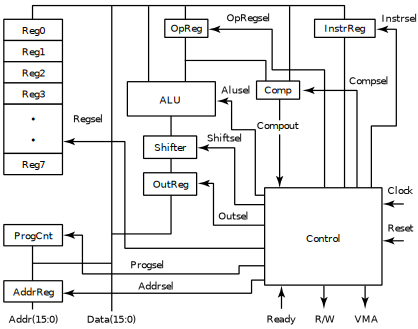
\includegraphics[scale=1.1]{perry-cpu}
	\caption[Bāzes prototipa uzbūves bloku diagramma.]
	        {Bāzes prototipa uzbūves bloku diagramma \cite[290.~lpp.]{Perry-VHDL}.}
	\label{fig:perry-cpu}
\end{figure}

D.~Perija procesors (turpmāk tekstā ,,bāzes prototips'')
ir vienkāršs 16 bitu procesors ar klasisku trīsstāvokļu 
centrālo datu kopni \cite{Flynn-arch}\cite{Heath}, un ar visām pamata
komponentēm (sk.~\ref{fig:perry-cpu}~att.), kas nodrošina bāzes prototipa
spēju izpildīt instrukcijas no tā instrukciju kopas.

\subsection{Iekšējā datu kopne} \label{sec:perry-bus}
	Bāzes prototipa arhitektūra paredz kopēju, trīsstāvokļu iekšējo datu kopne
	(sk.~\ref{fig:perry-cpu}~att.).
	Šāda kopnes uzbūve ir elektriski vienkārša, un ir shematiski viegli uztverama
	(sk.~\ref{fig:multidrop}~att.). Bet šāda uzbūve pieprasa kopnes
	,,arbitrēšanu'', t.i.,~nepieciešams
	nodrošināt, ka tikai viena no kopnei pievienotajām ierīcēm ir aktīvs devējs,
	kamēr pārējo ierīču izvadiem jābūt augstas impedances režīmā, kā arī
	jānodrošina, lai pareizā ierīce (vai ierīces) šos datus nolasītu no kopnes.

	\begin{figure}[thb]
		\centering
		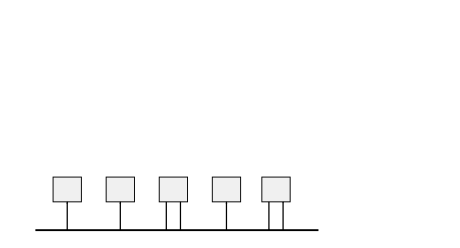
\includegraphics[scale=1.25]{multidrop}
		\caption{Kopējas trīsstāvokļu datu kopnes shēma.}
		\label{fig:multidrop}
	\end{figure}

	Galvenā problēma šādas kopnes izmantošanai sintezējama kodola izstrādei ir
	fakts, ka vairums (vai pat visas) FPGA neatbalsta iekšēju trīsstāvokļu
	loģiku, ko var secināt no fakta, ka neviena no apskatītajām FPGA neatbalsta
	loģisko bloku konfigurāciju ar trīsstāvokļu izejām
	\cite[18.~lpp.]{FusionFAQ}\cite{SmartFusionFabric}\cite{Xilinx7}.
	Tas nozīmē, ka pat, ja sintēzes rīks atbalsta šādas kopnes HDL aprakstu, tas
	ģenerēs ievērojami sarežģītāku struktūru, kas emulētu trīsstāvokļu datu kopni.

	Alternatīvas kopnes uzbūvē ir ķēdes savienojumi vai maršrutējams tīkls.
	Maršrutējami tīkli ir sarežģītas uzbūves un pieprasa tikpat sarežģītu
	kontroles loģiku. Savukārt, ķēdes savienojumi ir pietiekami vienkārši,
	tādēļ tiek izvēlēti par risinājumu.

	\begin{figure}[thb]
		\centering
		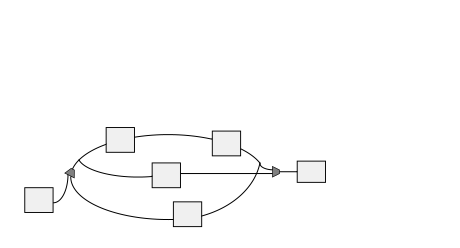
\includegraphics[scale=1.25]{chain}
		\caption{Vienvirziena cirkulāra ķēde ar atzarojumiem.}
		\label{fig:chain}
	\end{figure}

	Visai komplicēta ķēdes savienojumu struktūra ir redzama \ref{fig:chain}~attēlā,
	bet kas idejiski atbilst risinājuma rezultātam. 
	Ar ķēdes savienojumiem datu pārraide notiek vienā virzienā,
	tādējādi nav nepieciešamas divvirzienu pieslēgvietas, bet ir nepieciešamas
	atsevišķas pieslēgvietas datu ievadei un izvadei. Noslēdzot sazarojumus ar
	multipleksoriem zūd nepieciešamība pēc trīsstāvokļu loģikas.

	Ķēdes savienojumu priekšrocība ir arbitrēšanas vienkāršums. Ierīces uz kopnes
	jau ir savienotas ar datu saņēmejierīcēm, tādējādi vienīgā arbitrēšana ir
	datu plūsmas nodrošināšana (signalizēt datu nolasi) un sazarojumu noslēdzošo
	multipleksoru komutēšana.
	
	Ķēdes savienojumu kopnes ieguvums ir arī tā potenciālais datu caurlaides
	apjoms (\termEn{troughput}), kas ir ievērojami lielāks, jo ierīces nav
	savienotas pie viena mezgla, kas kopējā datu kopnē ir sastrēguma punkts
	(\termEn{bottleneck}). Datus dažādos ķēdes posmos var pārraidīt
	paralēli un kopnes atzaru datu pārraides ātrumi drīkst savā starpā 
	atšķirties.

	Tā kā procesora komponentēm nav nepieciešams komunicēt katrai ar katru, ir
	iespējams izveidot optimizētu kēžveida datu kopni, kur tieši savienotas ir tikai
	komponentes, starp kurām notiek tieša komunikācija. Kodolā iestrādāto
	risināju skatīt \ref{sec:databus}~nodaļā.

\pagebreak[3]
\subsection{Instrukciju kopa} \label{sec:perry-instr}
	Bāzes prototips paredz vienkāršu instrukciju kopu, ar konstanta garuma
	5 bitu operāciju kodiem. Instrukciju kopa ir tipiska \termEn{Load/Store}
	principa procesoru arhitektūrām. \termEn{Load/Store} princips nosaka, ka
	visas aritmētiskās, loģiskās, bīdes un salīdzināšanas darbības notiek
	ar vispārējā pielietojuma reģistru masīva reģistriem un datu apmaiņa ar
	operatīvo atmiņu notiek ar atmiņas nolases un ierakstes instrukcijām
	\cite[11.~lpp.]{Flynn-arch}	(sk.~\ref{sec:regArray}~nod.).
	Instrukcijas sadalāmas šādās grupās \cite[291.~lpp.]{Perry-VHDL}:
	\begin{itemize}
		\item \textbf{atmiņas nolases} (\termEn{load}) un \textbf{ierakstes}
			(\termEn{store}) instrukcijas, kuras
			veic datu apmaiņu starp reģistriem un operatīvo atmiņu;
		\item \textbf{zarošanās} instrukcijas, kas izmaina
			izpildāmā mašīnkoda (programmas) aktīvo pozīciju, un iekļauj
			nosacījuma un beznosacījuma zarošanās instrukcijas;
		\item instrukcijas, kuras veic \textbf{aritmētiskās} un 
			\textbf{bitu loģiskās} darbības ar reģistriem (operandiem);
		\item instrukcijas, kuras veic \textbf{bitu bīdes} reģistra
			(operanda) datiem.
	\end{itemize}
	
	Pēc autora domām, izmantotā instrukciju kopas izvēle ir racionāla, bet
	implementācija ir neoptimizēta. Pirmkārt, 5 bitu operācijas kods
	neefektīvi izmanto pieejamo 16 bitu mašīnvārdu
	(sk.~\ref{fig:5bit-opcode}~att.), efektīvāk būtu izmantot mainīga
	garuma operācijas kodu.
	\begin{figure}[thb]
		\centering
		
\includegraphics[scale=1.25]{perry-instr}
		\caption[5 bitu operācijas koda instrukcijas vārds.]
		        {5 bitu operācijas koda instrukcijas vārds \cite[292.~lpp.]{Perry-VHDL}.}
		\label{fig:5bit-opcode}
	\end{figure}
	
	Otrkārt, bāzes prototipa instrukciju operāciju kodi nes tikai kontroles
	iekārtai nozīmīgu informāciju un tiek pilnībā dekodēti dekodēšanas solī.
	Tas nozīmē, ka katrai instrukcijai nepieciešami savi, unikāli stāvokļi
	kontroles iekārtā (kas realizēta kā stāvokļu mašīna). Tā kā piem., 
	aritmētiskās instrukcijas (\texttt{ADD}, \texttt{SUB}, utt.)
	tiek izpildītas praktiski vienādi, iespējams veikt daļēju operācijas
	koda dekodēšanu un deleģējot atlikušā operācijas koda ,,dekodēšanu''
	ALU (sk.~\ref{sec:alu}~nod.), nododot tai nozīmīgu informāciju no
	operācijas koda. Tādējādi tiek panākta vienkāršāka dekodēšanas loģika un 
	mazāk stāvokļu kontroles iekārtā, jo pietiek ar vienu šablonveida
	izpildes stāvokļu ķēdi.
	
	Kodola realizācijai, autors ir pilnībā no jauna izveidojis instrukciju
	kopu, kas iekļauj visas iepriekš minētās instrukciju grupas, bet
	konkrētās instrukcijas un to izpildes implementācija, kas izmanto minētās optimizācijas,
	ievērojami atšķiras (sk.~\ref{sec:instrSet}~nod.).
	
	Izstrādājot kodolu arī veikta papildus arhitektūras specifiska
	optimizācija. Gan bāzes prototipa (sk.~\ref{fig:perry-cpu}~att.),
	gan izstrādātā kodola (sk.~\ref{fig:cpu-rev3}~att.) uzbūvē ALU un
	,,bitu bīdes iekārta'' atrodas uz viena signālceļa, kas nozīmē, ka
	izpildot gan bīdes, gan aritmētiskās instrukcijas dati tiek pārvadīti
	caur abām ierīcēm. Šo arhitektūras īpašību var izmantot izveidojot
	instrukciju, kas var veikt abas operācijas vienlaicīgi.
	Šādi kodolā implementēta \mnem{AR} instrukcija (sk.~\ref{sec:AR}~nod.).
	Tas arī nozīmē, ka visas aritmētiskās un bīdes instrukcijas ir izsakāmas
	ar šo ,,šabloninstrukciju'' vēl vairāk vienkāršojot kontroles iekārtas
	dekodēšanas loģiku un instrukciju izpildes stāvokļus.
	
\subsection{Komparators} \label{sec:perry-comp}
	Bāzes prototipā izmantotais komparators (sk.~\ref{fig:perry-comp}~att.),
	kura uzdevums ir salīdzināt	divus operandus (|a| un |b|), izvada
	rezultātu (|compout|) atkarībā pēc salīdzināšanas režīma signāla uz |sel|
	\cite[309.~lpp.]{Perry-VHDL}.
	\begin{figure}[thb]
		\centering
		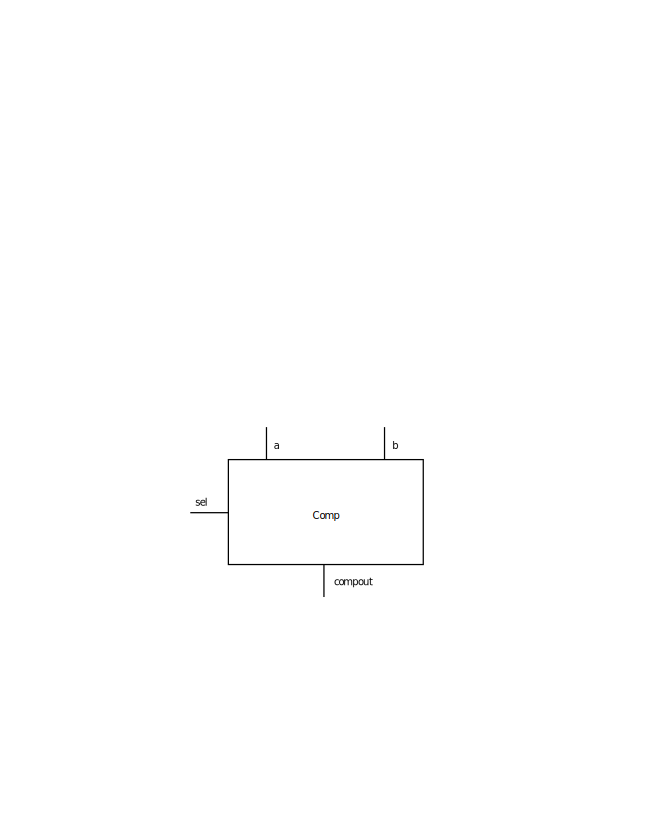
\includegraphics[scale=0.9]{perry-comp}
		\caption[Bāzes prototipa komparators.]
		        {Bāzes prototipa komparators \cite[309.~lpp.]{Perry-VHDL}.}
		\label{fig:perry-comp}
	\end{figure}
	
	Tiek definēti seši salīdzināšanas režīmi:
	\begin{itemize}
		\item operandu vienādība (|EQ|), kur |compout| ir |1|, ja |a|$=$|b|;
		\item operandu nevienādība (|NEQ|), kur |compout| ir |1|, ja |a|$\neq$|b|;
		\item operands |a| stingri lielāks (|GT|), kur |compout| ir |1|, ja |a|$>$|b|;
		\item operands |a| nestingri lielāks (|GTE|), kur |compout| ir |1|, ja |a|$\geq$|b|;
		\item operands |a| stingri mazāks (|LT|), kur |compout| ir |1|, ja |a|$<$|b|;
		\item operands |a| nestingri mazāks (|LTE|), kur |compout| ir |1|, ja |a|$\leq$|b|.
	\end{itemize}
	
	Šiem režīmiem eksistē ,,pretsakarības'', piem.~|EQ| ir pretējs |NEQ| un
	|GT| pretējs |LTE|, kas nozīmē ka šie režīmi ir redundanti. Izslēdzot
	redundantos režīmus iegūstam trīs: |LT|; |EQ|; |GT|, kas arī apzīmē
	trīs iespējamos operandu savstarpējos stāvokļus.
	Sekojot no matemātiskās aksiomas var pierādīt, ka
	\[
		\neg (a>b) \land (a \neq b) \iff (a<b)
	\]
	skaidri parādot, ka pārbaudot jebkurus divus stāvokļus, trešais
	nosakāms pēc izslēgšanas principa.
	\pagebreak[3]
	
	Tā vietā, lai nodotu vienu no sešiem pārbaudes režīmiem, komparatoru
	varam optimizēt, likvidējot režīmu pārslēgšanu vispār, un vienmēr izvadīt
	rezultātu no divu operandu savstarpējo stāvokļu pārbaudes.
	
	Kodola realizācijā izmantots ,,bezrežīmu'' komparators, kas 
	izvada divus signāla bitus, kas attiecīgi norāda 
	vai operands |a| ir vienāds ar |b| 
	un vai operands |a| ir lielāks par |b| (sk.~\ref{sec:comp}~nod.).
	Protams šāda implementācija nozīmē papildus loģiku kontroles iekārtā,
	bet tās implementācija ir visai vienkārša kā parādīts
	\ref{sec:branching}~nodaļā.

%\subsection{Kontroles iekārta}
%	\todo

	
	% Praktiskā daļa
	\clearpage
	\section{Mikrokontroliera kodola realizācija} \label{sec:cpu}
	Mikrokontroliera kodols pēc savas būtības un uzbūves ir procesors,
	kurš veic kalkulācijas un datu apmaiņu, nodrošinot mikrokontroliera
	programmas izpildi.
	Šajā darbā izstrādātais mikrokontroliera kodols ir 
	Fon-Neimaņa (\termEn{von~Neumann}) arhitektūras pro\-ce\-sors, kurš
	izmanto 16 bitu instrukcijas%
		\footnote{Instrukcijas var būt $N$-skaita 16 bitu vārdi. 
		Šajā darbā realizētas viena un divu vārdu instrukcijas.}
	un 16 bitu atmiņas adreses. Arī atmiņas vienība, kurai pieder unikāla
	adrese, ir 16 bitu plata. Kā Fon-Neimaņa procesoram, datu un
	programmkoda atmiņa ir kopēja un vienādi adresējama.[\todo]
	
	Kodola uzbūve ir daļēji balstīta uz D.~Perija (\termEn{D.~Perry}) grāmatas%
	\cite{Perry-VHDL} piedāvāto procesora reali\-zā\-ciju, 
	bet ar ievērojamām izmaiņām, galvenokārt, pilnībā no jauna izstrādāta 
	instrukciju kopa un vienvirziena,
	cirkulāra datu apmaiņas šina, atšķirībā no kopējas,
	trīs\-stāvokļu arbitējamas datu šinas.
	Galvenais šādas uzbūves datu šinas realizācijas iemesls
	ir izmantojamās \termEn{Actel} FPGA darba platformas trīs\-stāvokļu
	loģikas atbalsta \mbox{trūkums.\cite[18.~lpp.]{FusionFAQ}}
	
	Kodola saskarne ar pārējām mikrokontroliera komponentēm ir izveidota
	pēc iespējas vienkāršāka un platformas neatkarīga, lai nebūtu nepieciešams
	veikt izmaiņas kodola uzbūvē izmantojot to dažādās mikrokontroliera
	implementācijās, t.i.~kodola datu apmaiņa notiek izmantojot
	asinhronu atmiņas (RAM)	saskarni. Ar dažādām ierīcēm iespējama
	komunikācija iespējama, ja tiek izmantota saskarnes komponente, kas
	emulē RAM un multipleksē perifērās iekārtas pēc nododamās adreses.
	Tādējādi kodols	ir praktiski neatkarīgs no pārējās 
	mikrokontroliera implementācijas.
	Šī īpašība izmantota mikrokontroliera paraugimplementācijā.
	(sk.~\ref{sec:design}~un \ref{sec:mmu}~nod.)
	% TODO: 
	
	Instruckiju kopa ir izstrādāta no jauna un piedāvā vienkāršotu
	kopu līdzīgi RISC (\termEn{Reduced Instruction Set Computing})
	filo\-so\-fijai. Salīdzinot ar Perija realizāciju, ievērojami samazinātas
	nosacījuma zarošanās instrukcijas un instrukcijas pieejamie 16 biti
	tiek efektīvāk izmantoti ieviešot vektorizētus jeb dažāda garuma
	operāciju kodus. (detalizētākam aprakstam sk.~\ref{sec:instrSet}~nod.)
	
	
	%Tā kā \termEn{Actel} FPGA risinājums neatbalsta trīs stāvokļu
	%loģiku\cite[18.~lpp.]{FusionFAQ},
	%tad kopēju iekšējo datu šinu nav iespējams
	%izveidot. Tā vietā izveidota vienvirziena, nosacīti cirkulāra datu
	%apmaiņas līnija. Datu līnijas sazarojumi dažādu komponenšu 
	%komunikācijai realizēti ar multipleksoru palīdzību.
	
	%\begin{figure}[bhp]
	%	\centering
	%	\def\svgwidth{\textwidth}
	%	{\ttfamily\scriptsize\input{img/control.pdf_tex}}
	%	\caption{Procesora kontrole un atmiņas saskarne.}
	%	\label{fig:controlPipeline}
	%\end{figure}
	%
	%\begin{figure}[thp]
	%	\centering
	%	\def\svgwidth{\textwidth}
	%	{\ttfamily\footnotesize\input{img/aluPipeline.pdf_tex}}
	%	\caption{Aritmētikas un loģikas signālceļš un uzbūve.}
	%	\label{fig:aluPipeline}
	%\end{figure}
	
	\begin{figure}[thb]
		\centering
		\def\svgwidth{\textwidth}
		{\ttfamily\footnotesize\input{img/top-rev3-detail.pdf_tex}}
		\caption{Kodola uzbūve.}
		\label{fig:cpu-rev3}
	\end{figure}
	
	%\pagebreak[4]
	%\clearpage
	% TODO: Atmiņas izdalījums, 'von Neumann bottleneck' un kā DMA palīdz
	\subsection{Iekšējās datu šinas uzbūve} \label{sec:databus}
Izveidotajam procesoram ir sazarota, cirkulāra datu apmaiņas šina atšķirībā no kopējas,
trīsstāvokļu arbitējamas datu šinas. Šādai šinas uzbūvei ir vairākas
priekšrocības:
\begin{description}
	\item[Nav trīsstāvokļu loģika] \hfill \\
		Trīsstāvokļu loģikas trūkums atbrīvo no nepieciešamības izmantot
		trīsstāvokļu komponentes procesora iekšējā uzbūvē,
		samazinot realizācijas kompleksitāti.
	\item[Elektriskā drošība] \hfill \\ %TODO: Šitam citādāku nosaukumu?
		Nevienai no komponentēm pie šinas nevar tikt savienotas izejas,
		likvidējot iespējamo kaitējumu arbitācijas kļūdu rezultātā.
	\item[Mazāk vadības signālu] \hfill \\
		Šādai implementācijai nav nepieciešami nolases un rakstīšanas
		vadības signālu pāri katrai pievienotai ierīcei. Vienvirziena datu
		apmaiņa ļauj tikai pievadīt rakstīšanas vadības signālu%
		\footnote{Lai uzsvērtu šo vadības signālu nozīmi reģistru satura
			atjaunošanā, to nosaukumiem\\ pievienots -\texttt{Updt} piedēklis.}%
		, vai pat nevienu signālu kombinacionālo komponenšu gadījumā.
\end{description}

Viens no šādas šinas uzbūves trūkumiem var tikt uzskatīta nepieciešamība
multipleksēt signālus, bet pēc visu iespējamo datu apmaiņas scenāriju analīzes,
implementējamās instrukciju kopas ietvaros, tika noskaidrots ka --- 
pat ne tuvu --- katrai komponentei nepieciešama datu apmaiņa ar visām pārējām.
Konkrēti, tikai piecām komponentēm nepieciešama datu nolase no vairāk
nekā vienas citas.

%\todo % TODO: Tabula ar nepieciešamajiem savienojumiem
\begin{table}[hb]
	\centering
	\caption{Komponentes kurām nepieciešama ieejas multipleksēšana.}
	\label{tbl:muxes}
	\begin{tabular}{ll}
		\toprule
		Komponente & Ienākošie (multipleksējamie) dati\\ 
		\midrule
		Programmskaitītājs & Atmiņas ielase; ALU signālceļa dati\\
		Reģistru masīvs & Atmiņas ielase; ALU signālceļa dati\\
		ALU (pirmais operands) & Programmskaitītājs; Reģistru masīvs\\
		Komparators (pirmais operands) & Programmskaitītājs; Reģistru masīvs\\
		Adresācijas reģistrs & ALU signālceļa dati; Reģistru masīvs\\
		\bottomrule
	\end{tabular}
\end{table}

Apvienojot vienādos multipleksorus iegūstam optimizētu datu apmaiņas šinu
ar tikai trijiem \texttt{32>16} multipleksoriem. (sk.~\ref{fig:cpu-rev3}~att.)

%Galvenais šāda risinājuma iemesls
%ir izmantojamās \termEn{Actel} FPGA darba platformas trīs stāvokļu
%loģikas atbalsta \mbox{trūkums.\cite[18.~lpp.]{FusionFAQ}}
 %\clearpage 
	%\subsection{Procesora VHDL bibliotēka}
\todo
%\begin{singlespace}
	\lstinputlisting[language={[qucs]VHDL},float=h,%
					 caption={Procesora \texttt{cpu\_lib} pakas definīcija. (\texttt{cpu\_lib.vhd})},%
					 label=kb:cpulib,
					 basicstyle=\ttfamily\scriptsize]
		{code/cpu_lib.vhd}
%\end{singlespace}
	\clearpage
	\subsection{Komponentes}
Kā redzams procesora uzbūves shēmās
(\ref{fig:controlPipeline}.~un \ref{fig:aluPipeline}.~attēls), procesors
sastāv no dažādām apakš-komponentēm. Lai panāktu darba portabilitāti,%
\footnote{Iespējamu projekta izmantošanu dažādos izstrādes rīkos.}
komponentes aprakstītas RTL (\termEn{Register Transfer Level}) stila
VHDL apraksta kodā.

\subsubsection{Reģistri}
	Viena no vienkāršākajām komponentēm ir reģistrs. Tā funkcija ir uzglabāt
	viena vārda datus — šajā gadījumā 16 bitu vārda — un atjaunot to pēc
	pieprasījuma (ar \texttt{clk} signālu).
	
	\begin{figure}[bh]
		\centering
		%\def\svgwidth{7cm}
		\def\svgscale{1.25}
		{\ttfamily\scriptsize\input{img/sub-reg.pdf_tex}}
		\caption{Reģistrs.}
		\label{fig:reg}
	\end{figure}
	
	\noindent Procesorā ir vairāki atsevišķi reģistri ar savu nozīmi:
	\begin{description}
		\item[\texttt{PC} — Programmskaitītājs] \hfill \\
			Reģistrs, kas uzglabā adresi aktīvajai programmas pozīcijai,
			t.i.~parasti izpildāmās instrukcijas adresi. Secīgās programmas
			izpildes laikā \texttt{PC} tiek palielināts par 1%
			\footnote{Konkrētāk — \texttt{PC} tiek palielināts par
				izpildīto instrukcijas vārdu skaitu. (1 vai 2)},
			savukārt lēcieni (zarošanās)
			programmā realizēti pārrakstot programmskaitītāja saturu.
		\item[\texttt{instrReg} — Instrukciju reģistrs] \hfill \\
			Reģistrs, kurā ieraksta izpildāmo instrukcijas kodu.
			Nepieciešams, lai kontrole stāvokļa mašīna „neaizmirstu”
			izpildāmo operāciju un tās argumentus izpildot mikrokoda soļus.
		\item[\texttt{addrReg} — Atmiņas adresācijas reģistrs] \hfill \\
			Reģistrs, kurā ieraksta adresējamo atmiņas adresi tās nolasei
			vai ierakstei. Nepieciešams lai izvairītos no
			cirkulārās loģikas ielasot datus no atmiņas.
		\item[\texttt{opReg} — Operanda reģistrs] \hfill \\
			Reģistrs, kas uzglabā vienu no aritmētiskās/loģiskās darbības
			ope\-ran-diem, kamēr tiek iegūts otrs operands.
		\item[\texttt{outReg} — Izejas reģistrs] \hfill \\
			Reģistrs, kurā ieraksta aritmētiskās/loģiskās darbības rezultātu.
			Nepieciešams lai izvairītos no cirkulārās loģikas
			ierakstot rezultātu operatīvajos reģistros.
	\end{description}
	
	\begin{singlespace}
		\lstinputlisting[language={[qucs]VHDL},%float=pb,%
		                caption={Reģistra VHDL apraksts. (\texttt{reg.vhd})},%
		                label=kb:reg]
			{code/reg.vhd}
	\end{singlespace}

\pagebreak[3]
\subsubsection{Operatīvo reģistru masīvs}
	Operatīvie reģistri ir adresējama reģistru kopa, kura, atšķirībā no
	iepriekš apskatītajiem procesora specializētajiem reģistriem,
	ir pieejama	programmētājam tiešai modifikācijai.\\
	Tos sauc arī par vispārēja pielietojuma reģistriem, jo tiem nav noteikta specializēta
	nozīme, tā vietā programmētājs tos lieto pēc vajadzības, piem.~mainīgo
	uzglabāšanai.
	
	\begin{figure}[thp]
		\centering
		%\def\svgwidth{7cm}
		\def\svgscale{1.25}
		{\ttfamily\scriptsize\input{img/sub-regArray.pdf_tex}}
		\caption{Reģistru masīvs.}
		\label{fig:regArray}
	\end{figure}
	\begin{singlespace}
		\lstinputlisting[language={[qucs]VHDL},%float=pb,%
		                caption={Reģistru masīva VHDL apraksts. (\texttt{regarray2.vhd})},%
		                label=kb:regArray,%
		                emph={t_ram}]
			{code/regarray2.vhd}
	\end{singlespace}
	
	\pagebreak[2]
	Šajā realizācijā, reģistru masīvs vairāk līdzinās 8 vārdu operatīvajai
	atmiņai, bet netiek realizēta rakstīšanas vai lasīšanas režīma
	pārslēgšana. Tā vietā ir ieejas un izejas pieslēgvietas, kur
	ierakstītie dati tiek saglabāti un uzreiz izlikti uz izvadi.

\subsubsection{Multipleksors}
	Komponentēm, kurām datu šinā nepieciešams saņemt datus no dažādiem
	devējiem tiek multipleksētas, t.i.~devēju ieejas signāls tiek pārslēgts
	pēc nepieciešamības.
	
	Šim nolūkam izmantots multipleksors. Atšķirībā no citām procesora
	komponentēm multipleksors izveidots ar \termEn{Actel Libero}
	programmatūras pieejamo multipleksora makrosu, kura instancējamā
	entītijas definīcija parādīta \ref{kb:mux}.~koda blokā.
	
	\begin{figure}[thp]
		\centering
		%\def\svgwidth{7cm}
		\def\svgscale{1.25}
		{\ttfamily\scriptsize\input{img/sub-mux.pdf_tex}}
		\caption{2 ieeju multipleksors.}
		\label{fig:mux2}
	\end{figure}
	
	\begin{singlespace}
		\lstinputlisting[language={[qucs]VHDL},%float=pb,%
		                 caption={Multipleksora makrosa entītijas definīcija.},%
		                 label=kb:mux,%
		                 linerange={8-12},firstnumber=8]
			{code/gen/muxiitis.vhd}
	\end{singlespace}

\pagebreak[3]
\subsubsection{Aritmētiski loģiskā ierīce}
	Aritmētiski loģiskā ierīce jeb ALU ir viena no galvenajām,
	procesora definējošām
	komponentēm. Tās uzdevums ir veikt doto datu apstrādi, kā arī
	palielināt programmskaitītāju secīgas programmas izpildes nodrošināšanai.
	
	\begin{figure}[thp]
		\centering
		%\def\svgwidth{7cm}
		\def\svgscale{1.25}
		{\ttfamily\scriptsize\input{img/sub-alu.pdf_tex}}
		\caption{Aritmētiski loģiskā ierīce.}
		\label{fig:alu}
	\end{figure}
	
	Lai gan klasiski bīdes operācijas arī tiek realizētas Aritmētiski
	loģiskajā ierīcē, šajā gadījumā ALU veic tikai aritmētiskās un bitu
	loģikas darbības, atstājot bīdes operācijas „bitu bīdes loģiskjai ierīcei”
	(sk.~\ref{sec:shifter}.~nod.). Šāda sadalīšana ļauj veikt aritmētiskās
	un bīdes operācijas vienlaicīgi, uz ko balstās \mnem{AR} instrukcija
	(sk.~\ref{sec:AR}.~nod.~\pageref{sec:AR}.~lpp.)
	
	ALU realizēts ar asinhronu darbību, t.i.~izejas vērtība tiek izmainīta
	uzreiz bez kontroles signāla (takts) pievadīšanas.
	
	\begin{singlespace}
		\lstinputlisting[language={[qucs]VHDL},%float=pb,%
		                caption={ALU VHDL apraksts. (\texttt{alu.vhd})},%
		                label=kb:alu]
			{code/alu.vhd}
	\end{singlespace}

\pagebreak[3]
\subsubsection{Bitu bīdes loģiskā ierīce} \label{sec:shifter}
	Tā sauktā bitu bīdes loģiskā ierīce realizē bitu bīdes operācijas kuras
	šī procesora realizācijā ir izdalītas atsevišķi no ALU. Līdzīgi ALU
	realizācijai — darbojas asinhroni.

	\begin{figure}[thb]
		\centering
		%\def\svgwidth{7cm}
		\def\svgscale{1.25}
		{\ttfamily\scriptsize\input{img/sub-shift.pdf_tex}}
		\caption{Bitu bīdes loģiskā ierīce.}
		\label{fig:shift}
	\end{figure}
	
	\begin{singlespace}
		\lstinputlisting[language={[qucs]VHDL},%float=pb,%
		                caption={Bīdes ierīces VHDL apraksts. (\texttt{shifter.vhd})},%
		                label=kb:shifter,%
		                tabsize=3%,% TO REDUCE THE CODE WIDTH
		                ]
			{code/shifter.vhd}
	\end{singlespace}

%\clearpage
\pagebreak[3]
\subsubsection{Komparators} \label{sec:comp}
	Komparators jeb salīdzinātājs ir komponente, kas salīdzina 
	divus operandus un izvada tā vienādības vai nevienādības signālu.
	
	Šī komparatora implementācija ir minimizēta, kombinacionāla un nesatur
	kontroles signālus. Izvadīti tiek tikai divi biti, no kuriem viens
	norāda uz operandu vienādību vai nevienādību, savukārt otrs norāda
	vai operands \texttt{a} ir lielāks par \texttt{b} vai nav. Ar šo
	informāciju ir pilnīgi pietiekami, lai būtu iepējams realizēt visas
	nosacījuma zarošanās (\mnem{BRxx}) instrukcijas.
	\begin{figure}[thp]
		\centering
		%\def\svgwidth{7cm}
		\def\svgscale{1.25}
		{\ttfamily\scriptsize\input{img/sub-comp.pdf_tex}}
		\caption{Komparators.}
		\label{fig:comp}
	\end{figure}
	
	\begin{singlespace}
		\lstinputlisting[language={[qucs]VHDL},%float=pb,%
		                caption={Komparatora VHDL apraksts. (\texttt{comp.vhd})},%
		                label=kb:comp]
			{code/comp.vhd}
	\end{singlespace}

\pagebreak[3]
\subsubsection{Kontroles iekārta}
	Viena no procesora definējošām un iespējams sarežģītākajām komponentēm
	— kontroles iekārta ir tā kas nodrošina mikro-operāciju izpildi.
	Kontroles iekārta realizēta kā stāvokļa mašīna, kur katrs stāvoklis
	atbilst mikro-operācijai, un tātad tās VHDL apraksts ir uzskatāms par
	realizētā procesora mikrokodu.
	Kontroles iekārtas VHDL apraksts ir garš un sarežģīts, un tā daļas tiks
	izskatītas instrukciju darbības aprakstos.\\
	(Pilno kodu sk.~pielikumā~\ref{appx:control} \pageref{appx:control}.~lpp.)
	\begin{figure}[h!]
		\centering
		%\def\svgwidth{7cm}
		\def\svgscale{1.1}
		{\ttfamily\scriptsize\input{img/sub-control.pdf_tex}}
		\caption{Kontroles iekārta.}
		\label{fig:control}
	\end{figure}
 \pagebreak[3]
	\subsection{Instrukciju kopa} \label{sec:instrSet}
Instukciju kopa ir bāzēta uz RISC procesoru arhitektūrām, un
satur nedaudz vairāk par minimumu funkcionālam procesoram.
Instrukciju operāciju kodi ir vektoriski, lai efektīvi izmantotu pieejamo instrukcijas 
vārda garumu.

\begin{singlespace}\small
\begin{longtable}[c]{lp{20ex}lp{0.36\textwidth}}
	%\centering
	\caption{Instrukciju tabula.}\label{tbl:instructions}\\
	\toprule
	\textbf{Apz.} & \textbf{Mašīnkods} & \textbf{Argumenti} & \textbf{Operācija} \\
	\midrule \endfirsthead
	\caption[]{\nameref{tbl:instructions}~(turpinājums).}\\
	%\toprule
	\midrule
	\textbf{Apz.} & \textbf{Mašīnkods} & \textbf{Argumenti} & \textbf{Operācija} \\
	\midrule \endhead
	\multicolumn{4}{c}{Atmiņas datu apmaiņas instrukcijas}\\
	\midrule
	\mnem{LD} & 	\instr{01}{00}{}{XXXXXX}{XXX}{XXX}{} & \texttt{rD, rS} &
		\texttt{rD = *(rS)} \newline
		{\footnotesize Ielasa vārdu no RAM reģistrā \texttt{rD}} \\ \midrule
	\mnem{LDI} & 	\instr{01}{01}{}{XXXXXX}{XXX}{}{XXX} \newline
					\instr{}{}{}{}{}{XXXXXXXXXXXXXXXX}{} & \texttt{rD, C} &
		\texttt{rD = C} \newline
		{\footnotesize Ielasa konstanti reģistrā \texttt{rD}} \\ \midrule
	\mnem{ST} & 	\instr{01}{11}{}{XXXXXX}{XXX}{XXX}{} & \texttt{rD, rS} &
		\texttt{*(rD) = rS} \newline
		{\footnotesize Ielasa vārdu no RAM reģistrā \texttt{rD}} \\
	\midrule \pagebreak[3]
	\multicolumn{4}{c}{Aritmētika, loģika un bitu bīdes (un \mnem{AR} operācijas saīsnes)}\\
	\midrule
	\mnem{AR} & 	\instr{10}{}{}{}{XXXX}{XXX}{X}\instr{}{}{}{}{XXX}{XXX}{} & \texttt{kA, kS, rD, rS} &
		{\footnotesize Aritmētikas/bīdes instrukcija.} \\ \midrule
	\rule{0pt}{1em}\mnem{ADD} & \instr{10}{0000}{000}{X}{XXX}{XXX}{} & \texttt{rD, rS} &
		\verb|rD = rD + rS| \\ \midrule
	\rule{0pt}{1em}\mnem{SUB} & \instr{10}{0001}{000}{X}{XXX}{XXX}{} & \texttt{rD, rS} &
		\verb|rD = rD - rS| \\ \midrule
	\rule{0pt}{1em}\mnem{INC} & \instr{10}{1000}{000}{X}{XXX}{}{XXX} & \texttt{rD} &
		\verb|rD = rD + 1| \\ \midrule
	\rule{0pt}{1em}\mnem{DEC} & \instr{10}{1001}{000}{X}{XXX}{}{XXX} & \texttt{rD} &
		\verb|rD = rD - 1| \\ \midrule
	\rule{0pt}{1em}\mnem{AND} & \instr{10}{0010}{000}{X}{XXX}{XXX}{} & \texttt{rD, rS} &
		\verb|rD = rD & rS| \\ \midrule
	\rule{0pt}{1em}\mnem{OR} & \instr{10}{0011}{000}{X}{XXX}{XXX}{} & \texttt{rD, rS} &
		\verb+rD = rD | rS+ \\ \midrule
	\rule{0pt}{1em}\mnem{XOR} & \instr{10}{0100}{000}{X}{XXX}{XXX}{} & \texttt{rD, rS} &
		\verb|rD = rD ^ rS| \\ \nopagebreak \midrule
	\rule{0pt}{1em}\mnem{NOT} & \instr{10}{1010}{000}{X}{XXX}{}{XXX} & \texttt{rD} &
		\verb|rD = ~rD| \\ \midrule
	\rule{0pt}{1em}\mnem{CLR} & \instr{10}{1111}{000}{X}{XXX}{}{XXX} & \texttt{rD} &
		\verb|rD = 0| \\ \midrule
	\rule{0pt}{1em}\mnem{MOV} & \instr{10}{0101}{000}{X}{XXX}{XXX}{} & \texttt{rD, rS} &
		\verb|rD = rS| \\ \midrule
	\rule{0pt}{1em}\mnem{LSL} & \instr{10}{0101}{001}{X}{XXX}{XXX}{} & \texttt{rD} &
		\verb|rD = rS * 2| \newline
		{\footnotesize Loģiskā kreisā bīde (reizina ar 2)} \\ \midrule
	\rule{0pt}{1em}\mnem{LSR} & \instr{10}{0101}{010}{X}{XXX}{XXX}{} & \texttt{rD} &
		\texttt{rD = rS / 2} \newline
		{\footnotesize Loģiskā labā bīde (dala ar 2)} \\ \midrule
	\rule{0pt}{1em}\mnem{ROL} & \instr{10}{0101}{011}{X}{XXX}{XXX}{} & \texttt{rD} &
		{\footnotesize Bitu rotācija pa kreisi} \\ \midrule
	\rule{0pt}{1em}\mnem{ROR} & \instr{10}{0101}{100}{X}{XXX}{XXX}{} & \texttt{rD} &
		{\footnotesize Bitu rotācija pa labi} \\ \nopagebreak
	\midrule \pagebreak[3]
	\multicolumn{4}{c}{Plūsmas kontroles instrukcijas}\\
	\midrule
	\mnem{NOP} & 	\instr{00}{}{}{00000000000000}{}{}{} & nav &
		{\footnotesize „Ne-operācija”} \\ \midrule
	\mnem{HLT} & 	\instr{11}{0011}{}{XXXX}{}{}{XXXXXX} & nav &
		{\footnotesize Apstādina procesora darbību} \\ \midrule
	\mnem{JMP} & 	\instr{11}{0010}{}{XXXX}{}{}{XXXXXX} \newline
					\instr{}{}{}{}{XXXXXXXXXXXXXXXX}{}{} & \texttt{L} &
		\texttt{PC = L} \newline
		{\footnotesize Beznosacījuma lēciens.} \\ \midrule
	\mnem{BREQ} & 	\instr{11}{1000}{}{XXXX}{XXX}{XXX}{} \newline
					\instr{}{}{}{}{XXXXXXXXXXXXXXXX}{}{} & \texttt{rD, rS, L} &
		\texttt{if(rD==rS) PC = L} \\ \midrule
	\mnem{BRNQ} & 	\instr{11}{1011}{}{XXXX}{XXX}{XXX}{} \newline
					\instr{}{}{}{}{XXXXXXXXXXXXXXXX}{}{} & \texttt{rD, rS, L} &
		\texttt{if(rD!=rS) PC = L} \\ \midrule
	\mnem{BRGT} & 	\instr{11}{1010}{}{XXXX}{XXX}{XXX}{} \newline
					\instr{}{}{}{}{XXXXXXXXXXXXXXXX}{}{} & \texttt{rD, rS, L} &
		\texttt{if(rD>rS) PC = L} \\ \midrule
	\mnem{BRGE} & 	\instr{11}{1001}{}{XXXX}{XXX}{XXX}{} \newline
					\instr{}{}{}{}{XXXXXXXXXXXXXXXX}{}{} & \texttt{rD, rS, L} &
		\texttt{if(rD>=rS) PC = L} \\ \midrule
	\mnem{BRLT} & 	\multicolumn{2}{c}{subst.~\texttt{\textbf{BRGE} rS, rD, L}} &
		\texttt{if(rD<rS) PC = L}\\ \midrule
	\mnem{BRLE} & 	\multicolumn{2}{c}{subst.~\texttt{\textbf{BRGT} rS, rD, L}} &
		\texttt{if(rD<=rS) PC = L}\\
	\bottomrule
	\caption*{\fboxrule=0.75pt \framebox{\footnotesize
		\begin{tabular}{ll}
			\multicolumn{2}{c}{Mašīnkoda krāsu apzīmējumi} \\
			\textcolor{purple}{\rule[-2pt]{1em}{1em}} Operāciju grupas kods &
			\textcolor{blue}{\rule[-2pt]{1em}{1em}} \textcolor{cyan}{\rule[-2pt]{1em}{1em}}
				Operācijas „vektora” kodi \\[2pt]
			\textcolor{lightgray}{\rule[-2pt]{1em}{1em}} Ignorētie biti &
			\textcolor{OliveGreen}{\rule[-2pt]{1em}{1em}} \textcolor{Green}{\rule[-2pt]{1em}{1em}}
				Argumentu biti \\
		\end{tabular}
		}}
\end{longtable}
\end{singlespace}
\normalsize

\pagebreak
Kā redzams instrukciju tabulā, instrukcijas
ir sadalītas grupās vai nu pēc nozīmes, vai pēc izpildes līdzības. Šo
instrukciju realizācijas detaļas tiks apskatītas turpmākajās apakšnodaļās.

\subsubsection{\mnem{AR} instrukcija} \label{sec:AR}
	Lai gan \mnem{AR} instrukcijas apzīmējums ir saīsinājums no „aritmētika”
	un tā ir instrukcijas primārā nozīme, \mnem{AR} implementē visas
	aritmētiskās, loģiskās, bīdes operācijas, kā arī reģistru 
	apmaiņas \mnem{MOV} instrukciju. (sk.~\ref{tbl:instructions}.~tabulu)
	Šāda implementācija izmantota tāpēc, ka visas šīs instrukcijas tiek
	pārvadītas pa to pašu signālceļu. Tādējādi kontroles iekārta tiek
	vienkāršota, jo atsevišķās operācijas nav nepieciešams izšķirt.
	
	Kontroles signāli aritmētiskajai un bīdes ierīcei,
	kā argumenti jeb vektora kodi,
	tiek nodoti tieši no instrukcijas vārda, un kontroles iekārtā netiek
	interpretēti (jeb ir „necaurspīdīgi”). Izņēmums, gan ir 
	unārās un bezargumentu operācijas
	\mnem{INC}, \mnem{DEC}, \mnem{NOT} un \mnem{CLR}, kuru ALU
	vektora koda vecākais bits (\texttt{=1}) tiek interpretēts, lai izlaistu
	otrā operanda ielasi, tā samazinot nepieciešamo takts ciklu skaitu
	instrukcijas izpildei. (sk.~\ref{kb:ARdecode}.~koda bloku)
	
	\begin{singlespace}
		\lstinputlisting[language={[qucs]VHDL},%float=pb,%
		                caption={\mnem{AR} instrukcijas dekodēšana. (\texttt{control2.vhd})},%
		                label=kb:ARdecode,%
		                firstnumber=150]
			{code/gen/ardecode-snippet.vhd}
	\end{singlespace}


\subsubsection{Nosacījuma zarošanās instrukcijas} \label{sec:branching}
	Nosacījuma zarošanās ir vitāla īpašība pilnīgam procesoram. Programmēšanas
	valodu \texttt{if()} konstrukcija nav iedomājama bez
	nosacījuma zarošanās.
	
	Izstrādātais procesors par nosacījumu var izmantot divu reģistru
	vienā\-dības vai nevienādības, kur reģistru saturs tiek interpretēts, kā
	bezzīmes veseli skaitļi (t.i.~\texttt{unsigned~integer} tips).
	Šai salīdzināšanai atbilst \mnem{BRxx} instrukcijas
	(sk.~\ref{tbl:instructions}.~tabulu), un pašu salīdzināšanu veic komparators
	(sk.~\ref{sec:comp}.~nod.) kuram tiek pievadīti salīdzināmie operandi.
	
	\noindent Aparatūras līmenī realizētas četras zarošanās instrukcijas:
	\begin{itemize}
		\item \mnem{BREQ} — zaroties, ja operandi ir vienādi;
		\item \mnem{BRNQ} — zaroties, ja operandi nav vienādi;
		\item \mnem{BRGE} — zaroties, ja pirmais operands ir lielāks
			vai vienāds ar otro;
		\item \mnem{BRGT} — zaroties, ja pirmais operands ir stigri lielāks
			par otro.
	\end{itemize}
	Šo instrukciju operāciju kodi nav izvēlēti gluži patvaļīgi, tie tiek
	izmantoti loģiskā izteiksmē kopā ar komparatora signāliem, lai noteiktu
	zarošanās izpildes nosacījumus.
	
	\begin{figure}[thp]
		\centering
		%\def\svgwidth{7cm}
		\def\svgscale{1.5}
		{\ttfamily\input{img/karnaugh.pdf_tex}}\\
		\(
			f = \mathtt{\overline{A}E + BG + AG + AB\overline{E}}
		\)\\[1ex]
		(apzīmējumu nozīmi sk.~\ref{kb:branchTest}.~kodā)
		\caption{Zarošanās nosacījuma \termEn{Karnaugh} karte un formula.}
		\label{fig:branch-karnaugh}
	\end{figure}
	
	\begin{singlespace}
		\lstinputlisting[language={[qucs]VHDL},%float=pb,%
		                caption={Zarošanās nosacījuma pārbaudes funkcija (\texttt{control2.vhd})},%
		                label=kb:branchTest,%
		                linerange={61-69},firstnumber=61,
		                emph={state,branchTest},%
		                breaklines,breakatwhitespace,
		                basicstyle=\ttfamily\scriptsize]
			{code/control2.vhd}
	\end{singlespace}
	
	Atlikušās zarošanās instrukcijas \mnem{BRLT} un \mnem{BRLE} ir
	programmatūras līmeņa substitūcijas, jo to ekvivalentus var iegūt
	izmantojot attiecīgi \mnem{BRGE} un \mnem{BRGT} instrukcijas,
	apmainot salīdzināmos operandus vietām.
	
	
 %\clearpage %\pagebreak[3]
	% Man vajag revīziju cēsturi?
	%\subsection{Revīziju vēsture} \label{sec:cpu-revs}
%\todo

\begin{description}
	\item[Rev.~01] \hfill \\
		Par pamatu ņemta Perija grāmatas\citeet{Perry-VHDL} procesora
		realizācija. Atsevišķas komponentes izveidotas ļoti līdzīgi, bet
		kontroles iekārtas modelis un tam piekārtotā instrukciju tabula
		pilnībā izstrādāta no jauna.
	\item[Rev.~02] \hfill \\
		\termEn{Actel Fusion} FPGA nepiedāvā trīs-stāvokļu loģiku.\citeet{FusionFAQ}
		Tā rezultātā
		datu apmaiņas šina, pārveidota no kopējas arbitējamas 
		\termEn{multidrop} realizācijas pārveidota uz sazarotu vienvirziena
		pārraides ķēdi. Šāds solis pavildus ļāva arī likvidēt trīs-stāvokļu
		buferus un samazināt kontroles iekārtas signālu skaitu.
	\item[Rev.~03] \hfill \\
		Šī revīzija nav ienesusi fundamentālu izmaiņu procesora uzbūvē.
		(Izmaiņas sistēmas perifērijā skatīt
			\ref{sec:sys-revs}.~nod.~\pageref{sec:sys-revs}.~lpp.)
\end{description}
 %\pagebreak[3]
	
	% TODO?: Programmskaitītāja lokācija un PIC kods
 % Kodola uzbūve perifērija
	
	\clearpage
	\section{Mikrokontroliera realizācijas paraugs}
	Iepriekšējā nodaļā apskatītais mikrokontroliera kodols, lai gan centrālā
	komponente, bez papildus komponentēm ir praktiski nefunkcionāls, jo
	nav iespējams uzglabāt un pievadīt izpildāmās instrukcijas un veikt
	datu apmaiņu ar perifērām ierīcēm.
	
	%Vitāli svarīga komponente, praktiski jebkurā datoriekārtā, 
	%ir operatīvā atmiņa (RAM), kur
	%glabāt izpildāmo programmu, kā arī pirmsapstrādes, pēcapstrādes un 
	%apstrādes laika datus.
	
	Šī nodaļa apskata kā izveidotais kodols iekļaujas
	pilnīgā mikrokontroliera uzbūvē, piedāvājot	parauga implementāciju
	mikrokontrolierim. 
	Paraug\-implementācija paredzēta mikrokontroliera kodola 
	darbības demontrēšanai, kā arī kalpošanai par dokumentētu pamatu 
	turmākajām, iespējams specializētām implementācijām.
	
	\subsection{Implementācijas īpašības} \label{sec:design}
Izstrādājot mikrokontrolieri tika pieņemti vairāki lēmumi par tā uzbūvi,
veidojot specifikāciju kopu, uz kuras
balstās izstrādātātās mikrokontroliera komponentes.
Šim mikrokontrolierim ir sekojošas uzbūves īpašības:
\begin{itemize}
	\item \textbf{Vienota adrešu telpa}:
		mikrokontroliera kodols komunicē ar ārējām ierīcēm tikai caur
		atmiņas saskarni, bet ne obligāti šai ierīcei arī jābūt atmiņai.
		Tā vietā kopējai adrešu telpai tiek piekārtotas vairākas ierīces,
		katrai izdalot noteiktus adrešu apgabalus. Adrešu dekoderis veido saskarni,
		multipleksējot ierīces atkarībā no pieprasītās adreses
		(sk.~\ref{sec:mmu}~nod.).\pagebreak[1]
	\item \textbf{Aparatūras kontrolēta SPI saskarne}:
		atšķirībā no citiem mikrokontrolieriem ar SPI saskarni
		[\todo ], % FIXME: Citation needed
		šis mikro\-kontrolieris nodrošina aparatūras kontrolētu datu pārraidi,
		atšķirībā no programmatūras kontrolētu pārraidi ar
		\termEn{bit-banging} metodi%
		\footnote{Metode kurā takts signāls tiek ģenerēts izpildot programmu,
			pārraidot vienu bitu vienā vai vairākās instrukcijās.}.
		Tādējādi tiek vienkāršots programmkods SPI pārraidēm, un atbrīvots
		kodols citu darbību paralēlai izpildei.
	\item \textbf{Sāknēšana no ROM}:
		tā kā patstāvīgā atmiņa uz FPGA platformas ir ierobežota, tajā
		atrodas sāknēšanas (\termEn{boot}) programma,
		kura veic pamatprogrammas ielādi
		operatīvajā atmiņā no ārēja datu nesēja, šajā gadījumā no 
		SPI \termEn{Flash} atmiņas, kas pieejama uz darba platformas
		(sk.~\todo{}~nod.).
\end{itemize}

Tā kā adrešu telpai piekārtotas vairākas ierīces (sk.~\ref{fig:top-rev3}~att.),
rodas nepieciešamība pēc adreses dekodēšanas loģikas, kuru nodrošina
adrešu dekoderis jeb MMU, kas veido saskarni un 
aparatūras līmeņa abstrakcijas slāni, datu apmaiņai starp ierīcēm un kodolu.

\begin{figure}[tbhp]
	\centering
	\def\svgwidth{\textwidth}
	{\input{img/uC-sheem.pdf_tex}}
	\caption{Augšējā līmeņa blokshēma (rev.~03).}
	\label{fig:top-rev3}
\end{figure}

Tā kā perifērā mikrokontroliera daļa tieši izmanto realizācijas
platformas resursus, portabilitāte nav aktuāla un tiek brīvi izmantoti izstrādes rīka 
,,Actel Libero'' makrosi, kur tas nepieciešams vai potenciāli uzlabo
veiktspēju.
\FloatBarrier % Do not allow figures to "leak out"

	%\subsection{Simulētā shēma (rev.~02)}
Sākotnējā darba augšējā līmeņa sistēmas gala shēma paredzēta, kā
paškomplektējoša, tikai ar procesoru un atmiņu, 
kur no ārpuses tiek tikai dota takts (\texttt{CLOCK})
un atiestatīšanas signāls ($\overline{\texttt{RESET}}$). Darbības pārbaudei
tiek izmantotas izstrādes platformas piedāvātās diodes.

\begin{figure}[bhp]
	\centering
	\def\svgwidth{\textwidth}
	{\ttfamily\tiny\input{img/top-rev2.pdf_tex}}
	\caption{Augšējā līmeņa shēma (rev.~02).}
	\label{fig:top-rev2}
\end{figure}

Šī shēma tika veiksmīgi simulēta pirms sintēzes
(rezultātus sk.~\ref{appx:simulation}.~pielikumā),
bet tā nav korekti sintezējama, jo paredz RAM sākotnējos datus,
kurus sintēzes rīks ignorē.
Realitātē RAM dati tiek pazaudēti tikko tiek noņemts barošanas spriegums un
tātad pēc šādas shēmas nav iespējams saglabāt izpildāmo programmu.

\pagebreak[3]
%\subsubsection{Operatīvā atmiņa}
	Operatīvā atmiņa šeit realizēta ar divām vienvirziena datu apmaiņas
	šinām. Kontroles signāli izmantoti līdzīgi klasiskai trīs-stāvokļu
	divvirzienu datu šinas atmiņai, pielāgojoties procesora atmiņas
	saskarnei.
	
	\begin{singlespace}
		\lstinputlisting[language={[qucs]VHDL},%float=p,
		                caption={RAM VHDL entītija.},%
		                label=kb:ram-entity,%
		                linerange={7-13},firstnumber=7,
		                breaklines,breakatwhitespace]
			{code/mem.twoport.vhd}
	
		\lstinputlisting[language={[qucs]VHDL},%float=p,
		                caption={RAM VHDL arhitektūras apraksts (izgriezums).},%
		                label=kb:ram-trimmed,%
		                linerange={85-99},firstnumber=85,%
		                breaklines,breakatwhitespace]
			{code/mem.twoport.vhd}
	\end{singlespace}
	
	\noindent Pilno kodu skatīt \ref{appx:ram-code}.~pielikumā.
 \clearpage %\pagebreak[3]
	%\subsection{Papildinātā shēma (rev.~03)}

%Trešā sistēmas revīzija pievieno patstāvīgās atmiņas elementus sākotnējās
%programmas un datu uzglabāšanai. Šīs atmiņas ierīces piekārtotas kopējai
%adresācijas telpai, tādējādi rodas nepieciešamība pēc adreses dekodēšanas
%loģikas, kuru nodrošina MMU (\termEn{Memory map unit}).

\subsection{MMU — adrešu dekoderis} \label{sec:mmu}
	Adrešu dekoderis jeb MMU ir ierīce, kas atbild par adrešu telpas
	pārdalīšanu dažādām ierīcēm, kā arī nodrošina korektu komunikāciju
	ar šīm ierīcēm. MMU tādējādi var uzskatīt par mikrokontroliera kontroles
	iekārtu. MMU arī satur praktiski visu implementācijas un platformas
	specifisko kodu, kas tādējādi ir galvenā komponente kurā jāveic izmaiņas
	(vai pat jāimplementē no jauna) izmainot mikrokontroliera uzbūvi.
	
	MMU ar procesoru veido tādu pašu saskarni kā RAM,
	savukārt, piekārtojamo ierīču saskarne ir implementācijas definēta.
	Tādējādi MMU var uzskatīt par aparatūras līmeņa abstrakcijas slāni.
	
	\begin{figure}[thp]
		\centering
		\def\svgwidth{0.9\textwidth}
		{\ttfamily\small\input{img/remap.pdf_tex}}
		\caption{Adrešu telpas sadalījums.}
		\label{fig:memory-map}
	\end{figure}
	
	Adrešu telpas sadalījums (sk.~\ref{fig:memory-map}~att.) seko vienkāršiem pamatprincipiem:
	\begin{itemize}
		\item lielākie atmiņas bloki (konkrēti RAM) tiek novietoti augstākos
			atmiņas apgabalos, vienkāršojot dekodēšanas loģiku;
		\item patstāvīgo atmiņu (ROM) nepieciešams piekārtot ar sākuma
			adresi \texttt{0x0000}, jo tā saturēs sāknēšanas programmu,
			kuru nepieciešams izpildīt pēc mikrokontroliera atiestatīšanas
			(sk.~\ref{sec:rom}~nod.);
	\end{itemize}
	
	Papildus MMU arī satur konfigurācijas reģistru,
	ar kura palīdzību maināmi pieslēgto ierīču konfigurējamie parametri.
	Tas nepieciešams, lai lokalizētu šos izkliedētos parametru bitus
	adrešu telpai piekārtotā reģistrā. Šis konfigurācijas reģistrs arī kalpo
	par buferi novēlotai parametru izmaiņai, piem.,~SPI pārraides vārda garumu
	platumu nevar izmanīt pārraides laikā (sk.~\ref{sec:spi}~nod.).
	


\subsection{Sāknēšanas ROM} \label{sec:rom}
	Sāknēšanas ROM ir tikai nolasāmās, pastāvīgās atmiņas komponente, kura
	satur sāknēšanas (\termEn{boot}) programmu.
	Šīs programmas uzdevums ir ielādēt reālo izpildes programmu no
	ārēja datu avota. Parauga implementācijas testam tiek izmantota
	sāknēšanas programma, kas ielasa izpildāmo programmu no SPI \termEn{Flash}
	atmiņas (sk.~pielikumu~\ref{appx:boot}), kas atrodas uz izmantotās
	darba platformas (sk.~\ref{sec:devkit}~nod.).
	
	ROM realizēts ar Actel Fusion piedāvāto
	\texttt{FlashROM} makrosu, kas izmanto Actel Fusion FPGA
	speciālo FlashROM atmiņu \cite{FlashROM} (sk.~\ref{sec:devkit}~nod.).
	Maksimāli pieejamais ROM garums uz izmantojamās platformas ir
	1 kilobits jeb 64 vārdi \cite[12.~lpp.]{FusionGuide}. ROM mazā ietilpība ir
	galvenais iemesls, kādēļ mikrokontrolieris realizēts ar sāknēšanu.
	
	FlashROM adresējamā datu vārda garums ir 8 biti (1 baits),
	tādēļ realizēta speciāla nolases loģikas saskarne, kas nolasa divus
	baitus un kombinē tos vienā 16 bitu mašīnvārdā pirms to nodot MMU.
	Šeit FlashROM glabā 16 bitu vārdus ar jaunāko baitu (LSB) 
	vispirms, bet nolases loģika šo niansi padara mazsvarīgu.
	
	Lai nodrošinātu korektu nolasi no FlashROM, bija nepieciešams
	modulēt FlashROM un nolases loģikas takts impulsa platumu.
	Šāda realizācija ir kompromiss, jo pagarina ROM nolases laiku, bet
	nodrošina pret nestabilitāti ,,skriešanās problēmas'' dēļ, kas bija
	novērojama mikrokontroliera darbības simulācijas laikā (pirms korekcijām).
	
	\begin{figure}[tbh]
		\centering
		\def\svgwidth{\textwidth}
		{\ttfamily\small\input{img/rom-access.pdf_tex}}
		\caption{Laika diagramma datu vārda nolasei no ROM.}
		\label{fig:rom-time-diag}
	\end{figure}
	
	\pagebreak[2]
	Nolases loģika datu nolasi no FlashROM veic vairākos soļos (sk.~\ref{fig:rom-time-diag}~att.):
	\begin{enumerate}[\hspace*{\parindent}1)]
		\item paceļot ROM izvēles signālu |rom_sel|, tiek iespējota nolases
			loģika un uzsākts nolases cikls;
		% FIXME: Is this right?
		\item paceļot nolases loģikas takti |fetch_clock| 
			tiek nodrošināta korekts adreses signāls;
		\item pie lecošās |rom_clk| frontes FlashROM nolasa pievadīto adresi,
			bet dati izejā nav definēti;
		\item FlashROM izvada datus pie krītošās |rom_clk|	frontes;
		\item pie |fetch_clock| krītošās frontes ROM dati tiek ielasīti
			pagaidu reģistrā --- tiek nolasīts vecākais baits, 
			2.--5.~solis tiek atkārtots arī jaunākā baita nolasei;
		\item nolasot jaunāko baitu tiek pacelts |ready| signāls
			(nav uzrādīts attēlā), pēc kura kodols (vai MMU) datus var
			nolasīt un atiestatīt |rom_sel| signālu.
	\end{enumerate}
	
	

\subsection{Operatīvā atmiņa} \label{sec:ram}
	Operatīvā atmiņa jeb RAM ir galvenā izpildes laika datu uzglabāšanas
	atmiņa. Tā kā kodols ir Fon~Neimaņa arhitektūras procesors
	(sk.~\ref{sec:cpu}~nod.), RAM tiek izmantots gan izpildāmās
	programmas mašīnkoda, gan datu uzglabāšanai.
	
	RAM realizēts ar \texttt{RAM4K9} makrosu, kas izmanto specializēto
	RAM, kas pieejams uz Actel Fusion FPGA \cite{RAM4K9}.
	Tādējādi tiek
	efektīvāk izmantoti FPGA resursi, jo nav nepieciešams izmantot
	programmējamos loģiskos blokus.
	
	Actel Fusion FPGA uzbūves un \texttt{RAM4K9} makrosa
	definīcijas dēļ, RAM ir sadalīts divos blokos \cite{RAM4K9}. 
	%Tā kā platums un garums
	%ir konfigurējami ir vairākas iespējas RAM sadalījumam.
	Katrs no abiem blokiem satur 6144 vārdus,
	kopā sastādot 12288 vārdu lielu RAM.
	
	%\todo ?
	

\clearpage
\subsection{Adrešu telpai piekārtotā ievade/izvade}
	Adrešu telpā arī piekārtotas ievades un izvades komponentes,
	kuras nodrošina saskarni ar sistēmas perifēriju. Adrešu telpā šīm
	komponentēm izvietoti datu apmaiņas un konfigurācijas reģistri.
	
	\subsubsection{Vispārējas nozīmes ievades/izvades pieslēgvietas}
		Vispārējas nozīmes ievades/izvades pieslēgvietas jeb GPIO ir svarīga
		mikrokontroliera sastāvdaļa, kas ļauj saņemt un nodot signālus
		pieslēgvietām pievienotajām ierīcēm.
		
		GPIO pieslēgvietas apvieno kopās, kuras sauc par portiem. Tipiski, bet
		ne obligāti, porta platums (atsevišķo pieslēgvietu skaits) ir vienāds
		ar mašīnvārda garumu (šeit~16). Porta platums nevar pārsniegt
		mašīnvārda garumu, jo tad viss ports nav nolasāms, tādēļ, ka dati
		neietilpst datu pārvades kopnē. Tā vietā mikrokontrolierī iestrādā
		vairākus GPIO portus.
		
		\begin{figure}[th]
			\centering
			\def\svgwidth{0.9\textwidth}
			{\ttfamily\footnotesize\input{img/gpio.pdf_tex}}\\
			\makebox[0.9\textwidth][r]{kur $N$ ir GPIO porta platums bitos}
			\caption{GPIO porta uzbūve.}
			\label{fig:gpio}
		\end{figure}
		
		Izstrādātā GPIO porta uzbūves pamatā ir
		bidirekcionālo buferu kopa, kura realizēta ar $N$ skaita
		\texttt{BIBUF} makrosa instancēm, kur $N$ ir porta platums,
		un divi $N$ garuma reģistri \texttt{DDRx} un \texttt{WRRx},
		no kuriem \texttt{DDRx} kontrolē pieslēgvietu darbības virzienu un
		\texttt{WRRx} uzglabā izvadāmo vārdu (pieslēgvietām, kas ir izvades režīmā).
		
		Gan \texttt{DDRx}, gan \texttt{WRRx} ir lasāmi un pārrakstāmi.
		Pieslēgvietu satura nolasīšanai ir tikai lasāms ,,virtuālais reģistrs''%
		\footnote{Dati, kas nolasāmi kā reģistrs, kaut gan (mikrokontroliera iekšienē)
			neeksistē fizisks reģistrs datu uzglabāšanai.}
		\texttt{RDx}.
	
	Šajā mikrokontroliera paraugā realizēts viens 4 pieslēgvietu ports, kas
	pievienot uz darba platformas esošajām diodēm.
	
	\clearpage %\pagebreak[3]
	\subsubsection{SPI saskarne} \label{sec:spi}
		SPI (\termEn{Serial Peripheral Interface Bus}) ir sinhrona seriālās
		datu pārraides saskarne, ar vienpusēju plūsmas kontroli pēc
		\termEn{Master/Slave} modeļa.
		%[\todo{}] % FIXME: Citation needed. 
		SPI ir \termEn{de facto}%
		\footnote{Vispārēji pieņemts, bet neoficiāls.}
		standarts un ir liels skaits ierīču kas komunicē izmantojot SPI,
		tādējādi SPI ir vērtīga mikrokontroliera komponente.
		
		Darba ietvaros realizēta aparatūras kontrolēta paralēlā uz SPI saskarne.
		Šī saskarne implementē SPI \termEn{master} pusi, tādējādi mikrokontrolieris
		vada SPI komunikāciju un saskarnes paralēlajā pusē ir arī izvietoti
		plūsmas kontroles signāli (sk.~\ref{fig:spi}~att.).
		
		\begin{figure}[thp]
			\centering
			%\def\svgwidth{7cm}
			\def\svgscale{1.25}
			{\ttfamily\scriptsize\input{img/sub-spi.pdf_tex}}
			\caption{SPI saskarnes ierīce.}
			\label{fig:spi}
		\end{figure}
		
		SPI saskarne izstrādāta, lai programmatūras līmenī tā būtu vienkārši
		izmantojama. Datu pārraide veicama ar \mnem{ST} instrukciju, ierakstot
		pārraidāmos datus speciālajā SPI datu reģistrā, kas tūlīt uzsāk datu
		apmaiņu. Šī pārraide notiek bez procesora kodola līdzdalības.
		Otras ierīces atgrieztos datus var atgūt vienkārši nolasot
		SPI datu reģistru (ar \mnem{LD} instrukciju). Pārraidāmo datu garumu
		ir iespējams konfigurēt datu apmaiņai pa baitam (8 biti) vai
		pa vārdam (16 biti).
		
		Realizētā SPI saskarnes iekārta izmanto divus 8 bitu bīdes reģistrus
		datu uzglabāšanai. Šo bīdes reģistru apvienojums atbilst SPI datu reģistram.
		Tipiski arī otra (\termEn{slave})
		ierīce izmanto līdzīgu bīdes reģistru, tādējādi tiek izveidots cilpveida
		bīdes reģistrs, kur atsevišķie bīdes reģistri, pēc vesela pārraides cikla,
		datus savā starpā apmaina. Pārraidīto bitu skaits tiek uzskaitīts
		ar iekšēju skaitītāju. 
		\begin{figure}[th]
			\centering
			\def\svgwidth{\textwidth}
			{\ttfamily\footnotesize\input{img/spi-tx.pdf_tex}}\\
			\caption{SPI pārraides laika diagramma.}
			\label{fig:spi-tx}
		\end{figure}
		Pārraide notiek vairākos soļos
		(sk.~\ref{fig:spi-tx}~att.):
		\begin{enumerate}[\hspace*{\parindent}1)]
			\item izpildot \mnem{ST} instrukciju, MMU paceļ |INIT|
				signalizējot, ka jānolasa jaunais pārraidāmais vārds, kurš
				tiek paralēlā režīmā ierakstīts bīdes reģistros;
			\item |INIT| kļūstot zemam, bīdes reģistri tiek pārslēgti
				seriālā režīmā un tiek uzsākta datu pārraide;
			\item pie lecošās takts signāla frontes gan \termEn{master},
				gan \termEn{slave} puses ierīce nolasa datu bitu;
			\item pie krītošās takts signāla frontes uz datu apmaiņas
				signālvadiem tiek uzlikts nākamais bits;
			\item tiek atkārtota 3.~un 4.~darbība pārējiem datu bitiem;
			\item apmainot pēdējo datu bitu, tiek pacelts |READY|
				signalizējot, ka datu vārda apmaiņa ir pabeigta, un no
				\termEn{slave} ierīces
				saņemtais vārds ir nolasāms no |PDO| pieslēgvietas;
		\end{enumerate}
		
		%\todo ? % SPI mode 0
		
		SPI saskarne parauga mikrokontrolierī izmantota
		komunikācijai ar SPI \termEn{Flash} atmiņu,
		kura pieejama uz izstrādes platformas \cite[43.~lpp.]{FusionGuide},
		kur tiek glabāta galvenā izpildāmā programma, kura sāknēšanas procesa
		laikā tiks pārvietota uz RAM (sk.~\ref{sec:rom}~nod.~un pielikumu \ref{appx:boot}).
 \pagebreak[3]
	\subsection{Revīziju vēsture} \label{sec:sys-revs}
%\todo

\begin{description}
	\item[Rev.~01] \hfill \\
		Kā RAM izmantota atmiņas realizācija ar 
		trīs-stāvokļu, divvirzienu datu šinu.
	\item[Rev.~02] \hfill \\
		Līdzīgi revīzijas izmaiņām procesora uzbūvē, arī atmiņa pārveidota,
		likvidējot trīs-stāvokļu šinu un tā vietā divas vienvirziena šinas
		datu ieejai un izejai. Kontroles signāli atstāti bez izmaiņām,
		tādējādi atmiņa vēljoprojām „emulē” trīs-stāvokļu datu apmaiņu,
		saglabājot procesora iespēju strādāt ar divvirzienu šinas atmiņu
		(papildus izmantojot virziena maiņas buferus).
	\item[Rev.~03] \hfill \\
		Šī revīzija veic fundamentālas izmaiņas sistēmas perifērijā,
		pievienojot patstāvīgo atmiņu un realizējot adrešu telpas
		piekārtošanu datu ievades/izvades ierīcēm ar MMU palīdzību.
		Šai arī paredz sistēmas \termEn{boot} procesu, kur izpildes
		programma tiek pārvietota izpildei uz operatīvo atmiņu no
		patstāvīgās atmiņas.
\end{description}

 % Sistēmas perifērija
	
	\clearpage
	\section{Izmantotā darba platforma un rīki} \label{sec:devkit}
\todo

	
	% Literatūras saraksts
	\bibliographystyle{ieeetr}
	%\renewcommand{\refname}%
	%	{\vspace*{-12mm}\section*{Izmantotā literatūra}\vspace*{-6mm}}
	\clearpage
	%\pagestyle{empty}
	{\raggedright
	\begin{thebibliography}{9}
		\addcontentsline{toc}{section}{\refname}
		\bibitem{VHSIC}
			Creasey~D.J.,
			\textit{Advanced Signal Processing}.\linebreak[1]
			London: Peter~Peregrinus, 1985. ISBN~0-86341-037-5
		
		\bibitem{Flynn-arch}
			%Michael J.~Flynn,
			Flynn~M.J.,
			\textit{Computer Architecture: Pipelined and Parallel Processor Design}.
			\linebreak[3]
			London: Jones~and~Bartlett, 1995. ISBN~0-86720-204-1
		
		\bibitem{Heath}
			%Steve Heath,
			Heath~S.,
			\textit{Embedded systems design}, 2\nd edition.\linebreak[3]
			Oxford: Newnes, 2003. ISBN~0-7506-5541-1
		
		\bibitem{VITAL}
			IEEE,
			\textit{IEEE 1076.4/D1, DRAFT Standard, VITAL ASIC Modeling Specification}.
			New York: IEEE, 2000.
		
		\bibitem{ieee-1364.1}
			IEEE,
			\textit{IEEE Std. 1364.1-2002, IEEE Standard for Verilog Register Transfer Level Synthesis}.
			New York: IEEE, 2002.
		
		\bibitem{Mealy-VHDL}
			%Bryan Mealy, Fabrizio Tappero,
			Mealy~B., Tappero~F.,
			\textit{Free Range VHDL}.
			2012. [tiešsaiste] \linebreak[2]
			Pieejams: \url{http://www.freerangefactory.org/dl/free_range_vhdl.pdf}\linebreak[2]
			\mbox{[skatīts on 2012.~gada 2.~maijā]}
		
		\bibitem{HDL}
			%Gaurav Mehta, Sridhar Kintali,
			Mehta~G., Kintali~S.,
			\textit{Hardware Description Languages}.\linebreak[2]
			Santa Barbra: University of California,
			2009.
		
		%\bibitem{von-Neumann}
		%	John von Neumann,
		%	\textit{First Draft of a Report on the EDVAC},\linebreak[2]
		%	University of Pennsylvania, 1945.
		
		\bibitem{Perry-VHDL}
			%Douglas L.~Perry,
			Perry~D.L.,
			\textit{VHDL: Programming by Example}, 4\nth edition. \linebreak[2]
			New York: McGraw-Hill, 2002. ISBN~0-07-140070-2
		
		\bibitem{Vivek-Verilog}
			%Vivek Sagadeo,
			Sagdeo~V.,
			\textit{The Complete Verilog Book}.\linebreak[2]
			Norwell: Kluwer Academic Publishers, 1998. ISBN~0-7923-8188-2
		
		\bibitem{vhdl-vs-verilog}
			Smith~D.J.,
			\textit{VHDL \& Verilog Compared \& Contrasted}. [tiešsaiste]\linebreak[2]
			Pieejams: \url{http://www.angelfire.com/in/rajesh52/verilogvhdl.html}
			\mbox{[skatīts on 2012.~gada 21.~maijā]}
		
		\bibitem{Kumar-Verilog}
			% Deepak Kumar Tala,
			Tala~D.K., \textit{Gate Level Modeling}. [tiešsaiste]\linebreak[2]
			Pieejams: \url{http://www.asic-world.com/verilog/gate.html}
			\mbox{[skatīts on 2012.~gada 24.~maijā]}
		
		\bibitem{Vahid-RTL}
			%Frank Vahid,
			Vahid~F.,
			\textit{Digital Design with RTL Design, VHDL, and Verilog}, 2\nd edition.\linebreak[2]
			New York: % Hell knows which city
			John Wiley \& Sons, 2011. ISBN~978-0-470-53108-2
		
		\bibitem{FusionGuide}
			Actel corp.,
			\textit{Fusion Embedded Development Kit User's Guide}. %\linebreak[2]
			%USA: Actel,
			2009.
		
		\bibitem{FlashROM}
			Actel corp.,
			\textit{Fusion FlashROM}, Application Note AC236. %\linebreak[2]
			%USA: Actel,
			2005.
		
		\bibitem{RAM4K9}
			Actel corp.,
			\textit{Fusion SRAM/FIFO Blocks}, Application Note AC237. %\linebreak[2]
			%USA: Actel,
			2005.
		
		\bibitem{FusionFAQ}
			Actel corp.,
			\textit{Synplify — Synthesis Frequently Asked Questions}. %\linebreak[2]
			%USA: Actel,
			2009.
		
		\bibitem{SmartFusionFabric}
			Microsemi corp.,
			\textit{SmartFusion FPGA Fabric User's Guide}.
			%USA: Microsemi,
			2011.
		
		\bibitem{Xilinx7}
			Xilinx,
			\textit{7 Series FPGAs Overview}.
			%USA: Xilinx,
			2012.
	\end{thebibliography}
	} % "End of \raggedright"
	
	\clearpage
	\begin{center}
	\phantomsection\addcontentsline{toc}{section}{Galvojums}
	\Large\bfseries Galvojums
\end{center}

Ar šo es, Jānis Šmēdiņš, galvoju, ka bakalaura darbs ir izpildīts patstāvīgi,
konsultējoties ar darba vadītāju. No svešiem pirmavotiem ņemtā informācija
ir norādīta ar atsaucēm, dati un definējumi ir uzrādīti darbā.
Šis darbs tādā vai citādā veidā nav nekad iesniegts nevienai
citai pārbaudījumu komisijai.

\vspace{3cm}
\noindent
\begin{minipage}{\textwidth}
	\raggedright
	2012.~gada \textcolor{gray}{\rule[-2pt]{2em}{1pt} \rule[-2pt]{10em}{1pt}}
	\hfill
	\textcolor{gray}{\rule[-2pt]{10em}{1pt}}\\[-1ex]
	\hfill\makebox[10em][c]{\tiny (paraksts)}
\end{minipage}

	
	\clearpage
	%\phantomsection\addcontentsline{toc}{section}{\appendixtocname}
	%\appendix
	\begin{appendices} % Pielikumu sākas šeit
	%\addappheadtotoc
	%\appendixtocname % Pievienot vārdu 'Pielikums' pie numura
	\section{Kontroles iekārtas pilnais kods} \label{appx:control}
\lstinputlisting[language={[qucs]VHDL},%
                caption={Kontroles iekārtas VHDL apraksts. (\texttt{control2.vhd})},%
                label=kb:control,
                emph={state,branchTest},%
                breaklines,breakatwhitespace,
                basicstyle=\ttfamily\scriptsize ]{code/control2.vhd}

\clearpage
\section{Atmiņas dekodera pilnais kods} \label{appx:mmu}
\lstinputlisting[language={[qucs]VHDL},%
                caption={Atmiņas dekodera VHDL apraksts. (\texttt{mmu.vhd})},%
                label=kb:mmu,
                %emph={state,branchTest},%
                breaklines,breakatwhitespace,
                basicstyle=\ttfamily\scriptsize ]{code/mmu.vhd}

%\clearpage
%\section{RAM pilnais kods} \label{appx:ram-code}
%\lstinputlisting[language={[qucs]VHDL},%
                %caption={RAM VHDL apraksts. (\texttt{mem.twoport.vhd})},%
                %label=kb:ram,
                %%emph={state,branchTest},%
                %breaklines,breakatwhitespace,
                %basicstyle=\ttfamily\scriptsize ]{code/mem.twoport.vhd}

\clearpage
\section{Simulācijas rezultāti (rev.~02)} \label{appx:simulation}
% MEMORY DUMP "language" definition
\lstdefinelanguage{memdump}
{
	keywordsprefix=@,
	comment=[l]{//}
}

\lstinputlisting[language={memdump},
                 caption={Atmiņas saturs pirms programmas izpildes.},
                 label=kb:mem-before,
                 basicstyle=\ttfamily\small,
                 firstline=4,firstnumber=4]{code/gen/before8.mem}

\lstinputlisting[language={memdump},
                 caption={Atmiņas saturs pēc programmas izpildes.},
                 label=kb:mem-after,
                 basicstyle=\ttfamily\small,
                 firstline=4,firstnumber=4]{code/gen/after8.mem}

\lstinputlisting[language={},
                 caption={Atmiņas satura izmaiņas.},
                 label=kb:mem-diff,
                 basicstyle=\ttfamily\small,]{code/gen/mem8.diff}

\begin{sidewaysfigure}
	\centering
	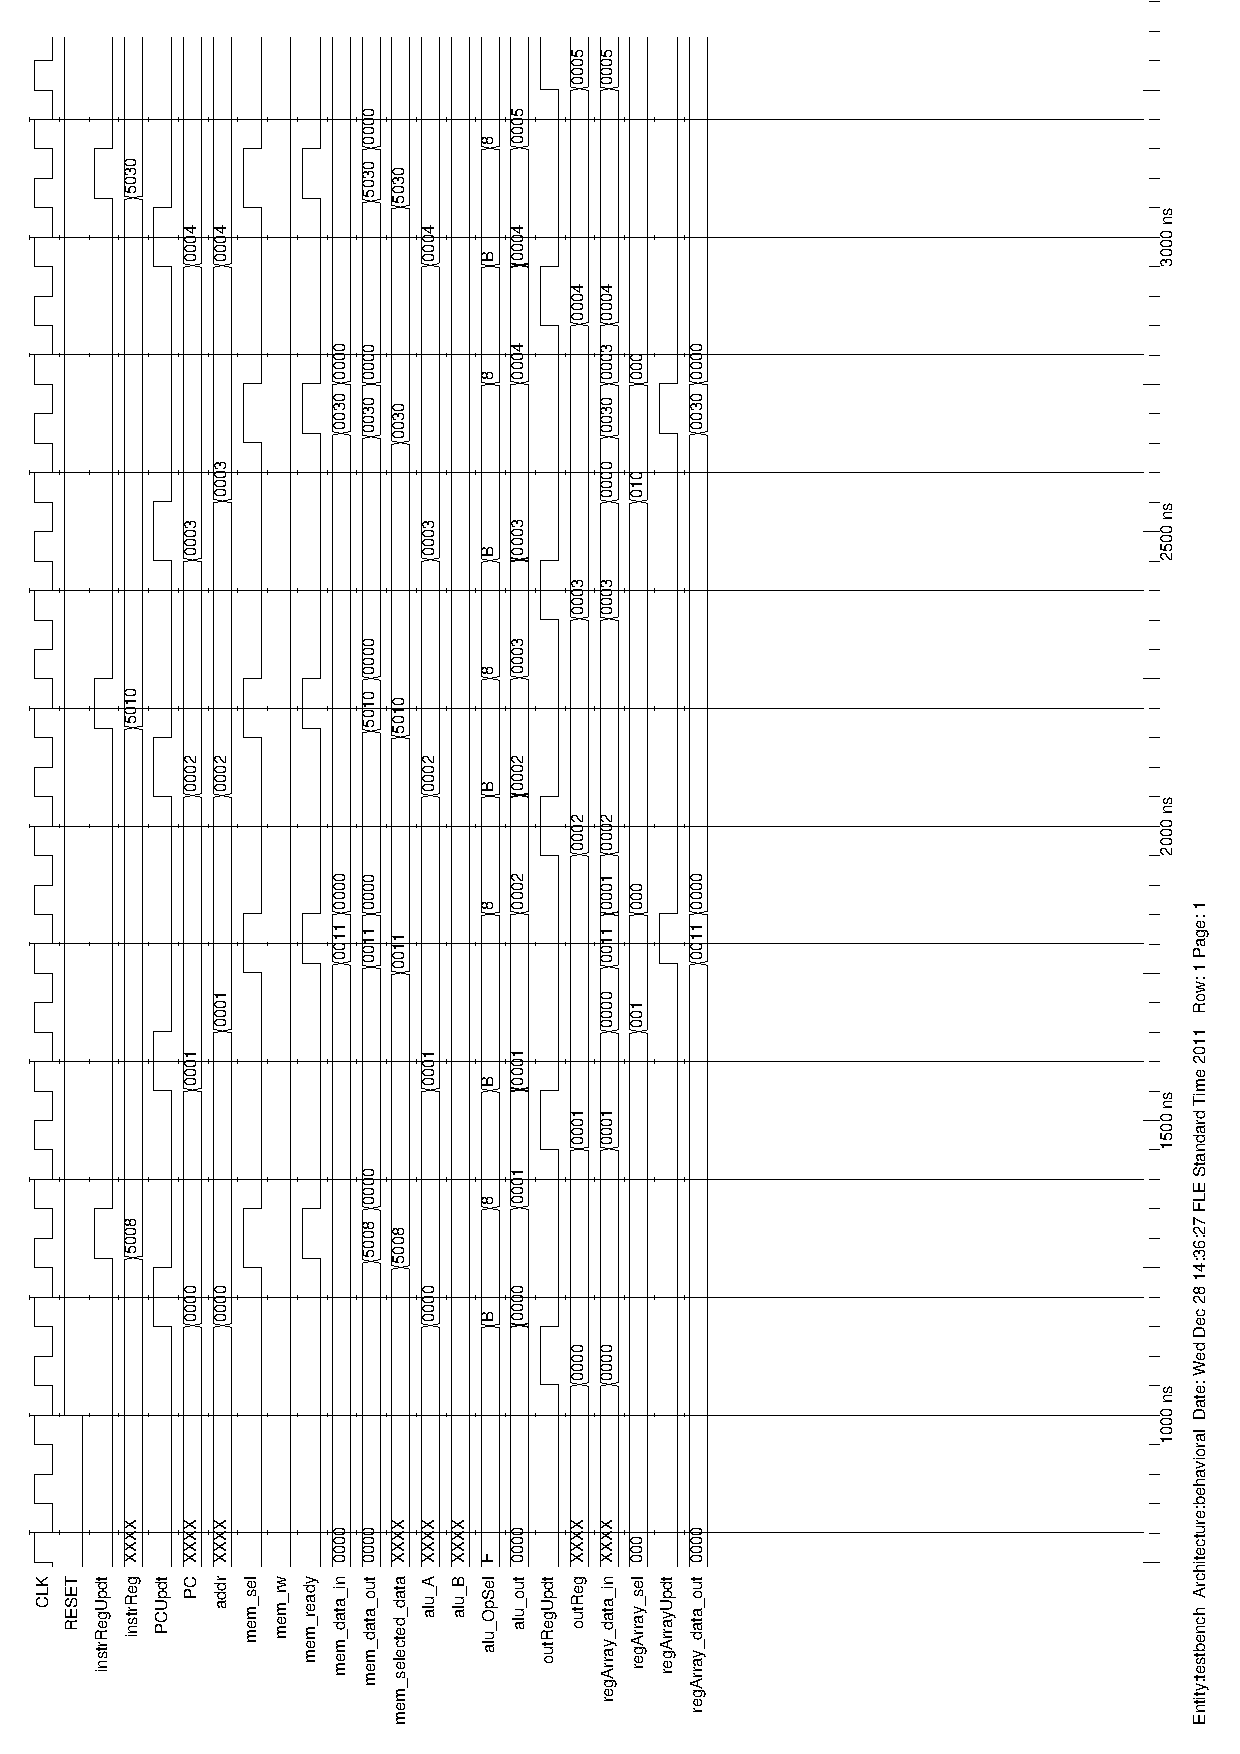
\includegraphics[trim = 0cm 0cm 8cm 0cm,clip,angle=-90,width=\linewidth]{sim0-init}\\
	\caption{Inicializācijas laika diagramma.}
	\label{fig:sim-init}
\end{sidewaysfigure}

\begin{sidewaysfigure}
	\centering
	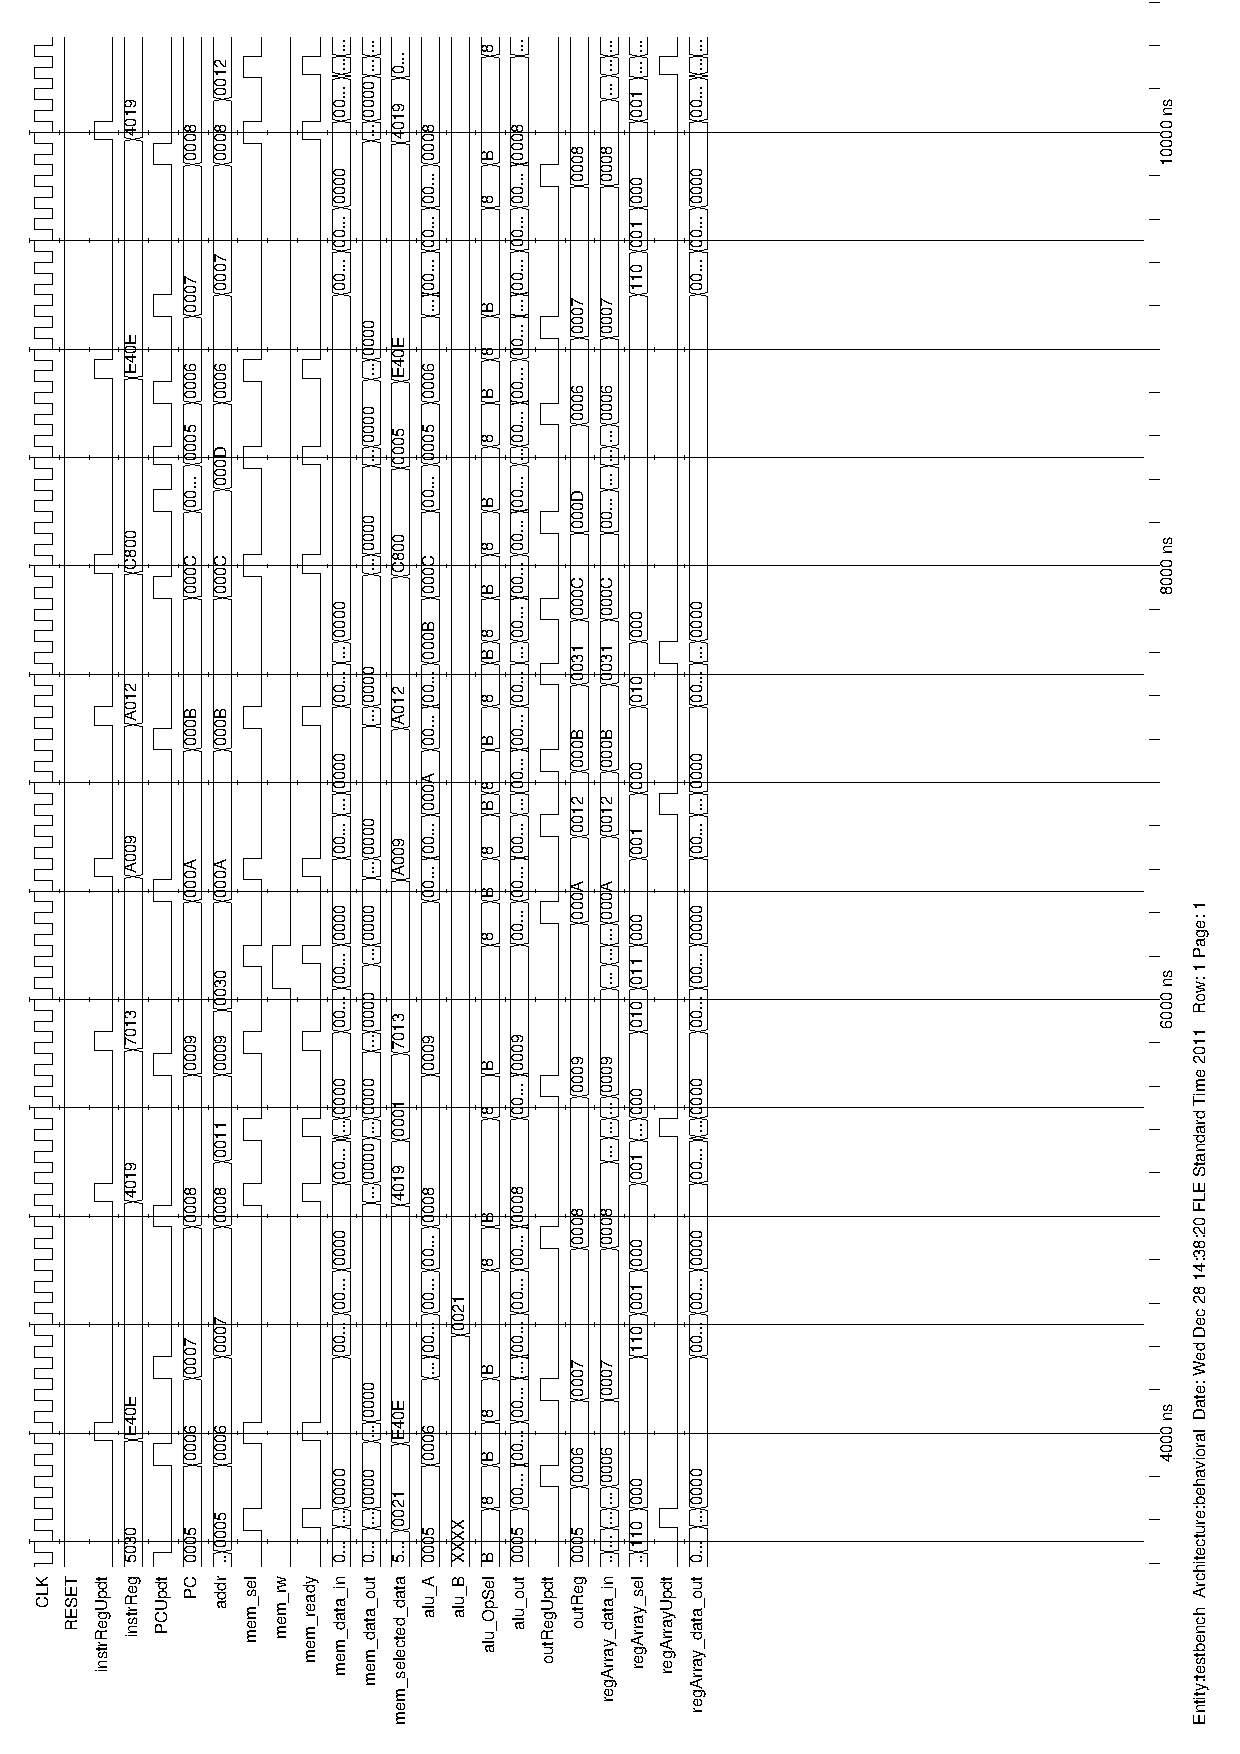
\includegraphics[trim = 0cm 0cm 8cm 0cm,clip,angle=-90,width=\linewidth]{sim0-cycle}\\
	\caption{Programmas cikla izpildes laika diagramma.}
	\label{fig:sim-cycle}
\end{sidewaysfigure}

\begin{sidewaysfigure}
	\centering
	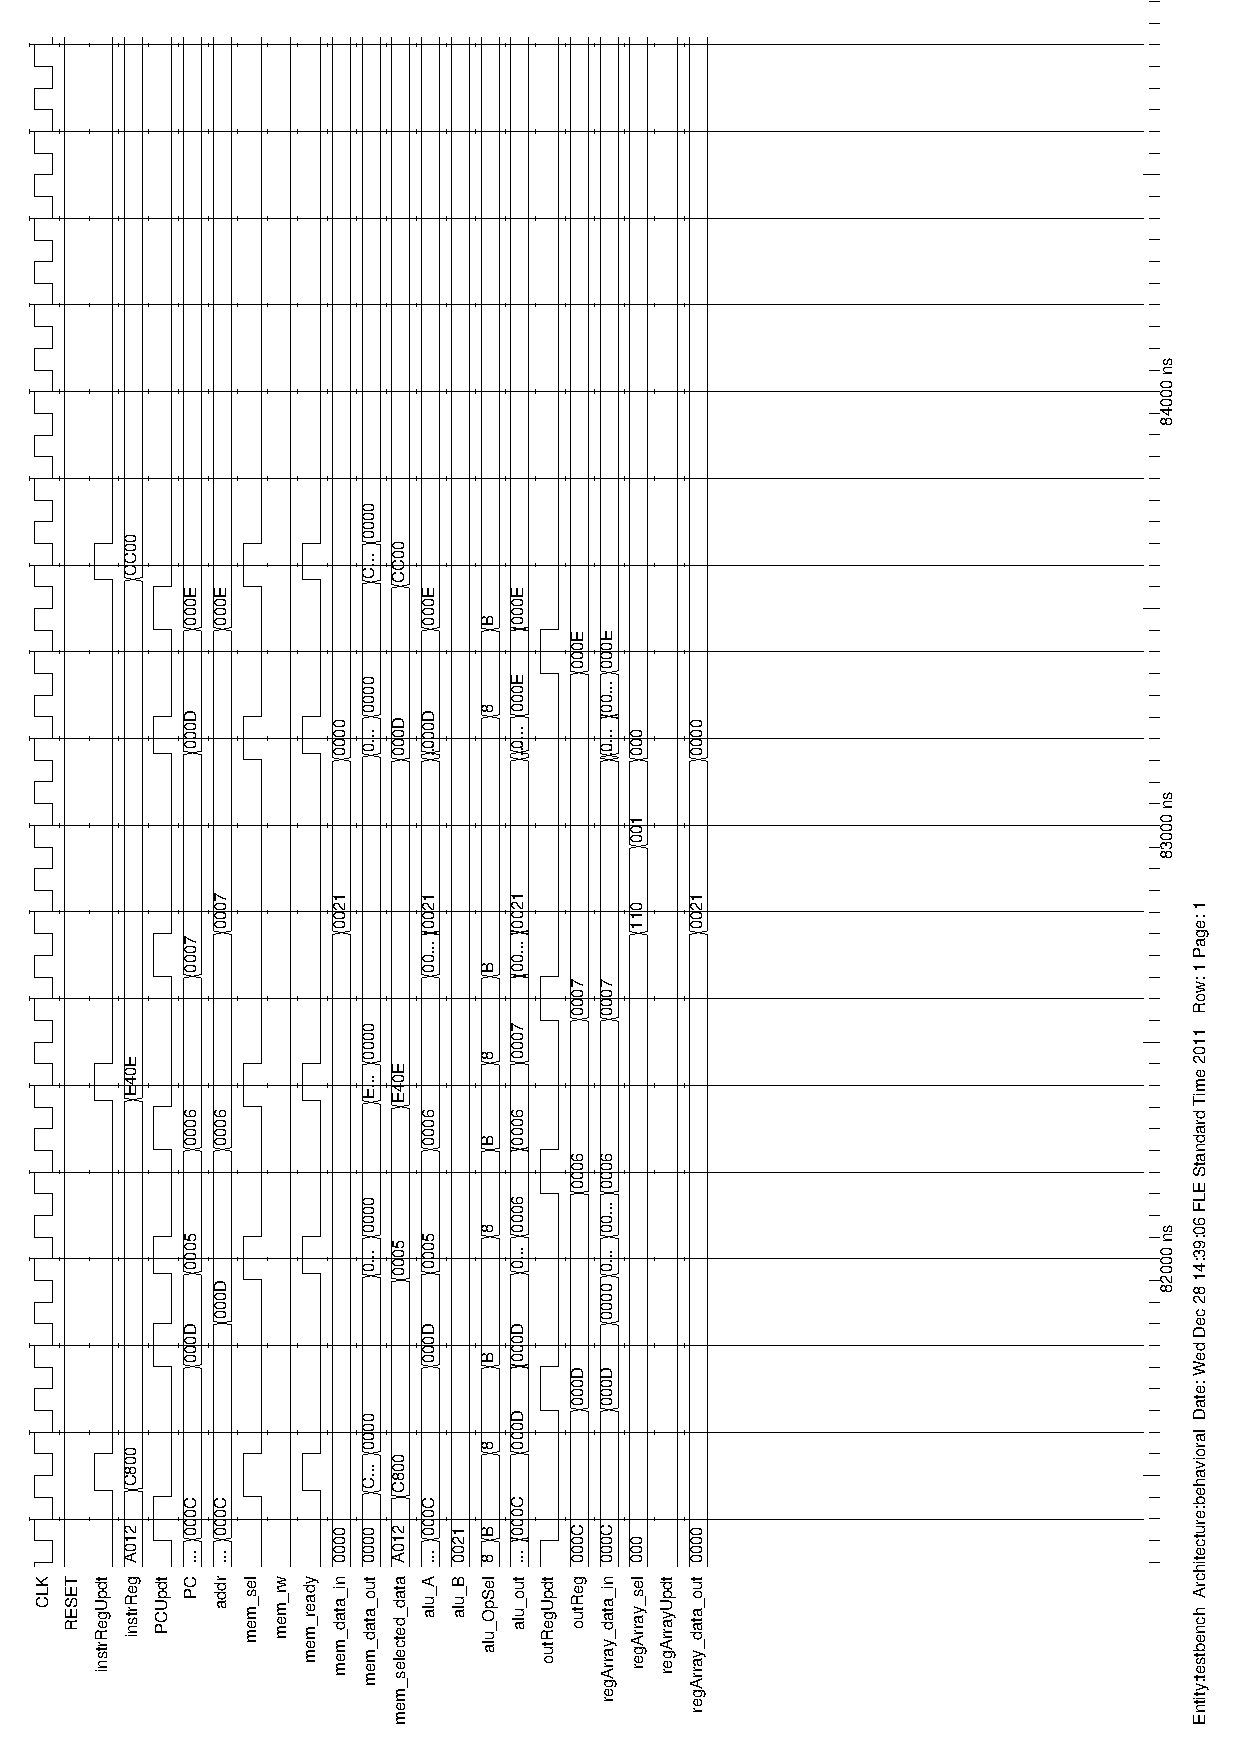
\includegraphics[trim = 0cm 0cm 8cm 0cm,clip,angle=-90,width=\linewidth]{sim0-halt}\\
	\caption{Programmas izpildes beigu laika diagramma.}
	\label{fig:sim-halt}
\end{sidewaysfigure}

\lstinputlisting[float=p,
                 language={JSI},
                 caption={Testa programmas asemblerkods.},
                 basicstyle=\ttfamily\scriptsize,
                 label=kb:copy-program]{code/gen/copy-noaccents.asm}

\clearpage
\section{Paraugimplementācijas asemblerkoda galvene (rev.~03)}
\lstinputlisting[%float=hp,
                 language={JSI},
                 caption={Galvene asemblera programmām (\texttt{JISonFUSIONr3.inc}).},
                 basicstyle=\ttfamily\scriptsize,
                 label=kb:asm-header]{code/JSIonFUSIONr3.inc}

\clearpage
\section{Sāknēšanas programma un simulācijas rezultāti (rev.~03)} \label{appx:boot}
\lstinputlisting[%float=hp,
                 language={JSI},
                 caption={Sāknēšanas programmas asemblerkods.},
                 basicstyle=\ttfamily\scriptsize,
                 label=kb:boot]{code/boot.asm}

\begin{sidewaysfigure}
	\centering
	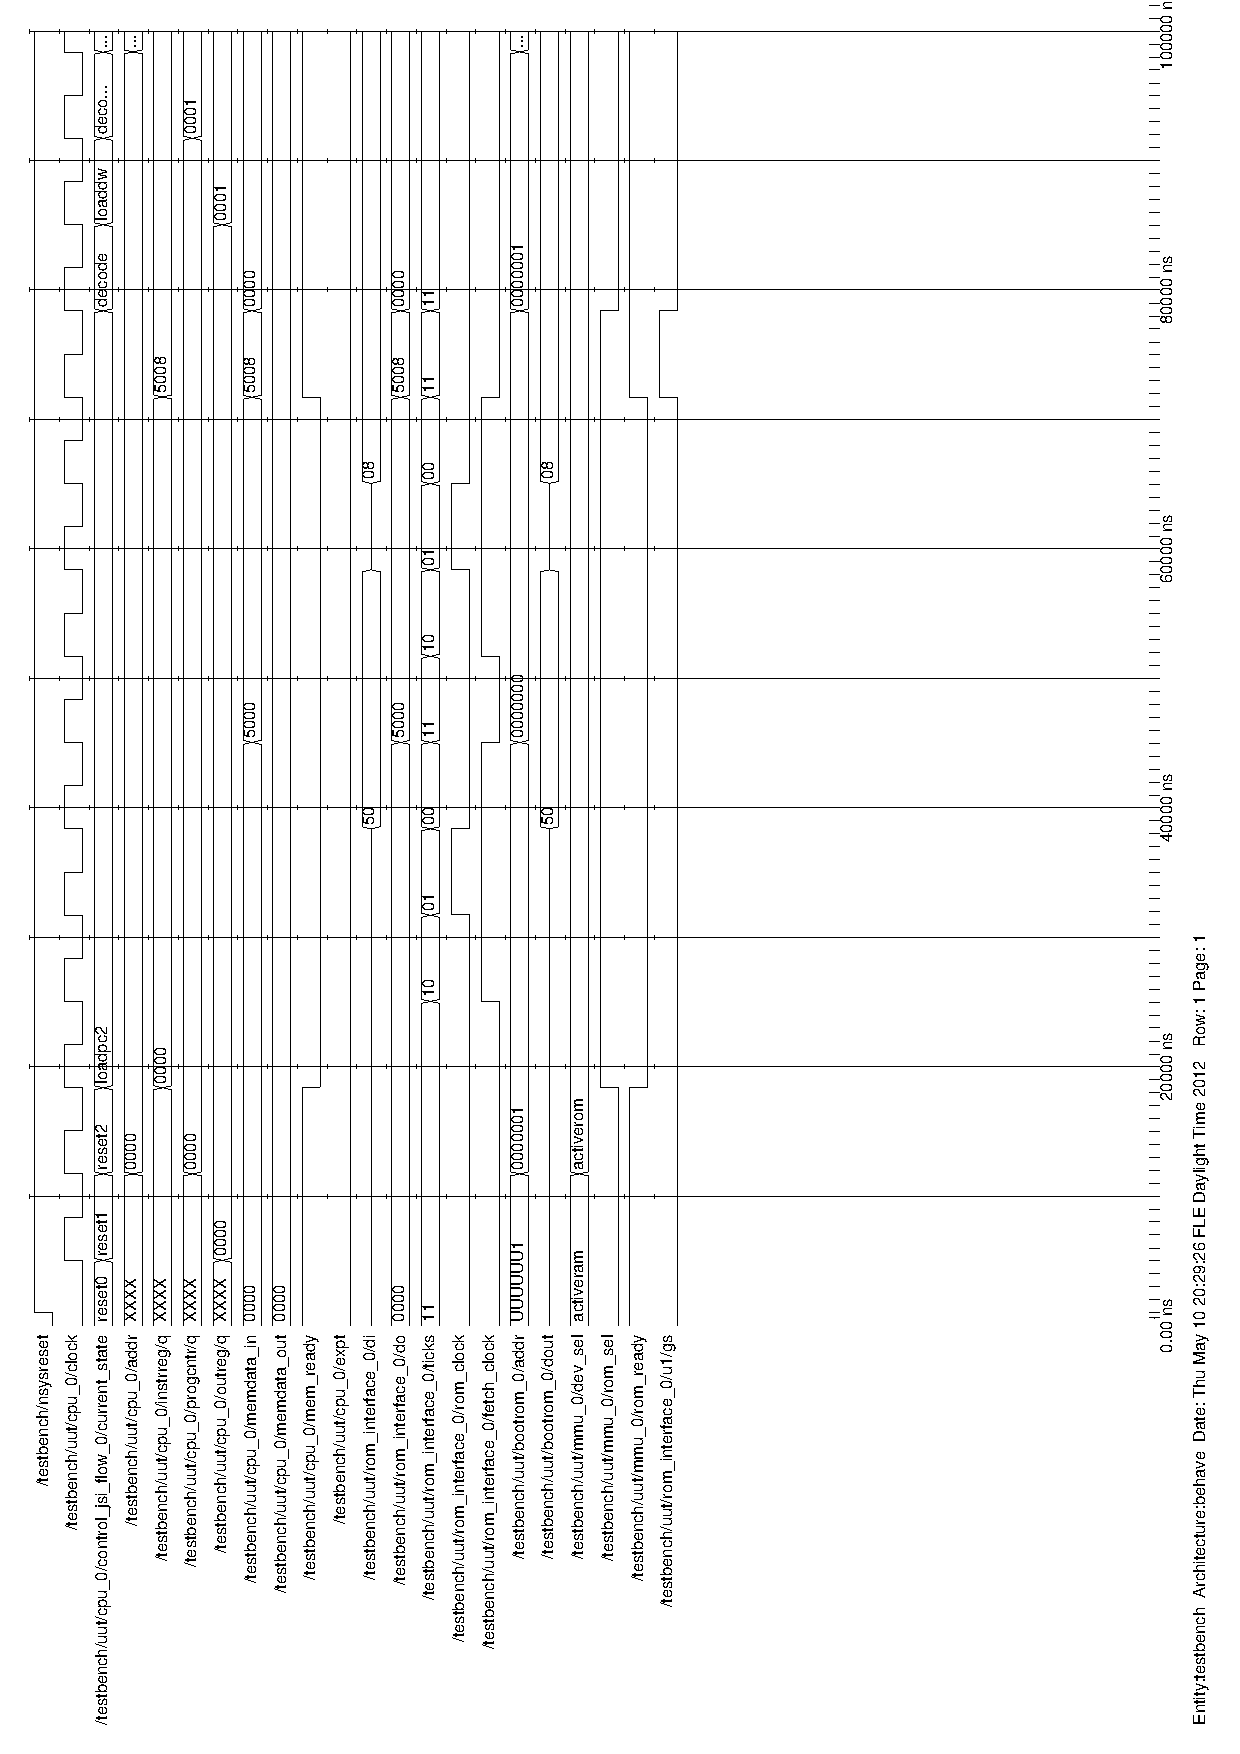
\includegraphics[trim = 0cm 0cm 8.75cm 0cm,clip,angle=-90,width=\linewidth]{sim1_init}\\
	\caption{Mikrokontroliera inicializācijas laika diagramma.}
	\label{fig:sim-boot}
\end{sidewaysfigure}

\begin{sidewaysfigure}
	\centering
	\includegraphics[trim = 0.5cm 0cm 3.25cm 0cm,clip,angle=-90,width=\linewidth]{sim3_tx}\\
	\caption{SPI \termEn{Flash} nolases komandas nosūtīšanas laika diagramma.}
	\label{fig:sim-spi-tx}
\end{sidewaysfigure}

\begin{sidewaysfigure}
	\centering
	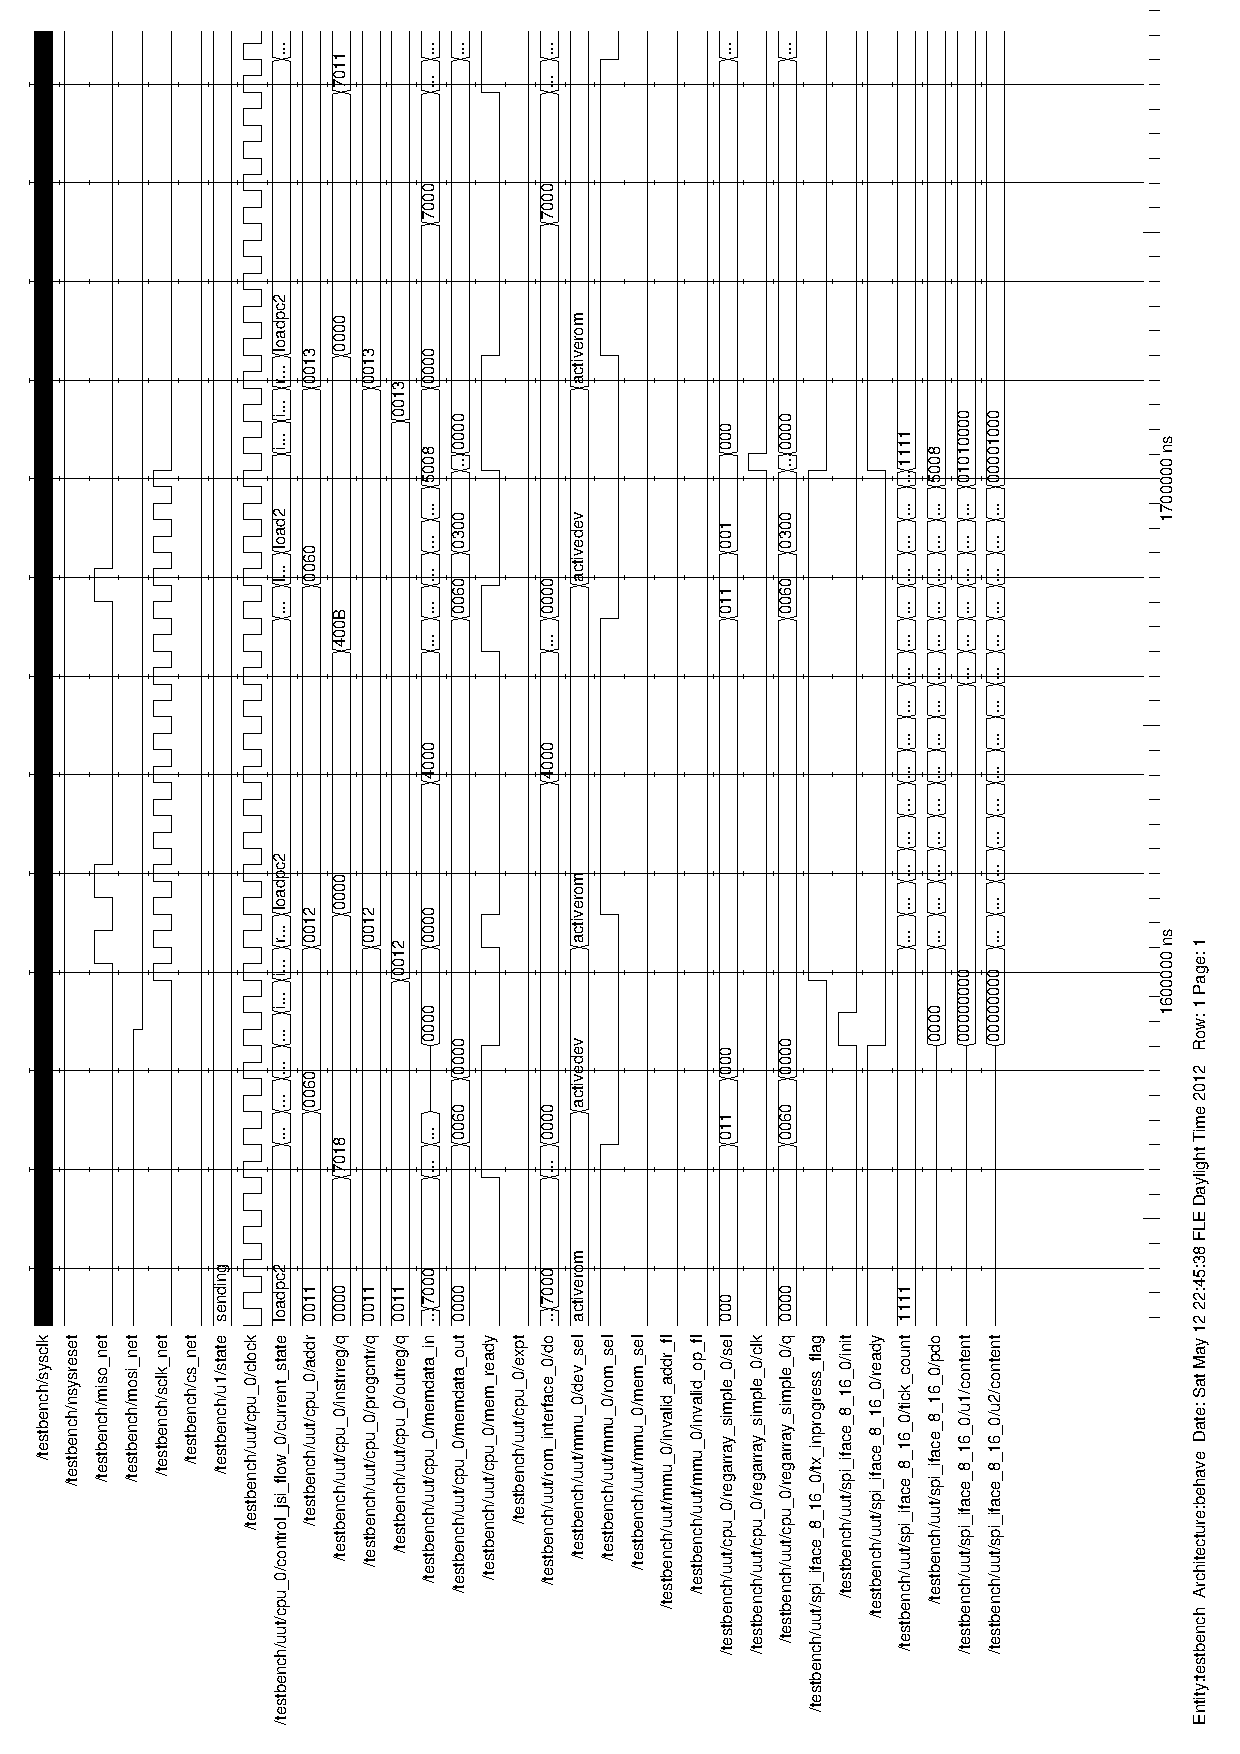
\includegraphics[trim = 0.5cm 0cm 3.25cm 0cm,clip,angle=-90,width=\linewidth]{sim3_rx}\\
	\caption{SPI \termEn{Flash} datu nolases cikla laika diagramma.}
	\label{fig:sim-spi-rx}
\end{sidewaysfigure}

	\end{appendices}
	
	\clearpage
	\vspace*{2cm}\raggedright
\thispagestyle{empty}
Bakalaura darbs aizstāvēts Gala pārbaudījumu komisijas sēdē\\[1cm]
2012.~gada \textcolor{gray}{\rule[-2pt]{3em}{1pt}\hspace{1ex}\rule[-2pt]{10em}{1pt}}\\[1em]
un novērtēts ar atzīmi \textcolor{gray}{\rule[-2pt]{10em}{1pt}}\\[1em]

\vspace{2cm}
\noindent Protokols Nr. \textcolor{gray}{\rule[-2pt]{3em}{1pt}}\\[1cm]

\noindent
Gala pārbaudījumu komisijas priekšsēdētājs\\[1cm]
\textcolor{gray}{\rule[-2pt]{20em}{1pt}}\\[-1ex]
\makebox[20em][c]{\tiny (paraksts)}


	
	
\end{document}
